\documentclass{article}
\usepackage{amsmath}
\usepackage{amssymb}
\usepackage{amsfonts}
\usepackage{mathtools}
\usepackage{mathrsfs}
\usepackage{amsthm}
\usepackage{bbm}
\usepackage{graphicx}
\usepackage{pgfplots}
\usepackage{tikz}
\usepackage{array}
\usetikzlibrary{shapes.geometric, calc}
\usetikzlibrary{intersections, calc}
\usepackage{geometry}

\title{Differential Equations - MATH246}
\author{Tom Mitchell}
\date{Conway - Fall 2024}

\begin{document}

\maketitle

\section*{Class Information}

\subsection*{Grading}
\begin{itemize}
    \item Matlab assignments — 18\% (6\% each)
    \item Quizzes (drop two lowest) — 17\%
    \item Two best in-class exams — 17\% each
    \item Worst in-class exam — 8\%
    \item Final exam — 23\%
\end{itemize}

\subsection*{Office Hours}
\begin{itemize}
    \item Monday: 2:00 PM - 3:00 PM (in person, Kirwin 2400)
    \item Tuesday: 1:15 PM - 2:30 PM (in person, Kirwin 2400)
    \item TBA: Zoom (online)
\end{itemize}

\subsection*{Exams}
\begin{itemize}
    \item 3 midterms and a final exam
\end{itemize}

\section*{Lecture 1, Tuesday 8/27/2024}

\section*{Course Overview: (Differential Equations)}

\section*{Chapter 0:}

A differential equation is an algebraic relation between functions, their derivatives, and independent variables.

\pagebreak

\textbf{Examples:}
\begin{itemize}
    \item \( \left(\frac{dx}{dt}\right)^2 + x \sin(t) = \cos(x) \) \hfill \textit{(Order = 1)}
    \item \( y'' + ty' + y = \cos(t) \) \hfill (Note: \(y' = \frac{dy}{dt})\)\textit{(Order = 2)}
    \item \( \frac{dy}{dt} \cdot \frac{dy}{ds} + y \frac{dz}{dt} = \sin(st) \) \hfill \textit{(Order = 1)}
\end{itemize}

\textbf{Order:} The order of a differential equation is the order of the highest derivative that appears.

\textbf{Notation:} For \( \frac{dy}{dx} \), we can write \( y' \) or \( \dot{y} \) (dot notation).

An ordinary differential equation (ODE) involves no partial derivatives, as opposed to a partial differential equation (PDE).

\textbf{Note:} This course only deals with ODEs.

\subsection*{Linearity of ODEs}

An ODE with function \( y \) and independent variable \( t \) is \textbf{linear} if it can be written as:

\[
a_n(t)y^{(n)} + a_{n-1}(t)y^{(n-1)} + \dots + a_1(t)y' + a_0(t)y = f(t)
\]

\textit{where \( y^{(n)} \) is the \( n \)th derivative of \( y \).}

\textbf{Examples:}
\begin{itemize}
    \item \( \left(\frac{dx}{dt}\right)^2 + x \sin(t) = \cos(x) \) \hfill \textit{(Not linear: \( \left(\frac{dx}{dt}\right)^2 \) and \( \cos(x) \))}
    \item \( y'' + ty' + y = \cos(t) \) \hfill \textit{(Linear)}
    \item \( y^{(4)} + y^{(2)} = 2 \) \hfill \textit{(Linear)}
\end{itemize}

\subsection*{Systems of ODEs}

A system of ODEs consists of multiple ordinary differential equations that are considered together:

\[
\left\{
\begin{array}{l}
\text{ODE} 1 \\
\text{ODE} 2 \\
\vdots \\
\text{ODE} n
\end{array}
\right.
\]

\section*{Chapter 1: Introduction}

\subsection*{Section 1: First-Order ODEs}

First-order ODEs can be complicated. We will focus on those that can be put into the standard form \(\boxed{\frac{dy}{dt} = f(t, y)}\).

\textbf{Example:} Consider the equation \(\frac{dw}{dz} = \frac{-z}{6w}\). This can be rewritten as:

\[
\frac{dw}{dz} = \frac{-z}{6w}
\]

A function \(Y(t)\) is a solution to \(y' = f(t, y)\) on the interval \((a, b)\) if:

\begin{itemize}
    \item \(Y(t)\) and \(Y'(t)\) exist on \((a, b)\),
    \item \(f(t, Y(t))\) exists on \((a, b)\), and
    \item \(Y'(t) = f(t, Y(t))\) on \((a, b)\).
\end{itemize}

\textbf{Example:} Consider the equation \(y'(t) = \frac{t}{y}\) with the solution \(Y(t) = \sqrt{4 - t^2}\).

To check this, calculate:

\[
Y'(t) = \frac{-t}{\sqrt{4 - t^2}}
\]

\(Y(t)\) is defined on the interval \([-2, 2]\), but \(f(t, Y(t)) = \frac{t}{\sqrt{4 - t^2}}\) is only defined for \((-2, 2)\), not at \(\pm 2\). Therefore, \(Y(t)\) is a solution on \((-2, 2)\), not on \([-2, 2]\).

\subsubsection*{Explicit Equations}

These are of the form \( y' = f(t) \).

The general solution is:

\[
y = \int f(t) \, dt = F(t) + C
\]

where \( F(t) \) is an antiderivative of \( f(t) \) (i.e., \( F'(t) = f(t) \)) and \( C \) is a constant.

\textbf{Example:} Consider the ODE

\[
\frac{dy}{dx} = 2x + 1
\]

The general solution is:

\[
y = x^2 + x + C
\]

\textbf{Graph for different values of \( C \):}

\begin{center}
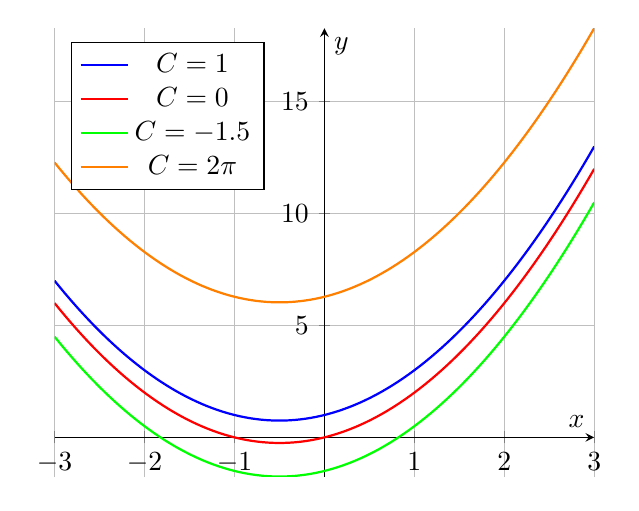
\begin{tikzpicture}
    \begin{axis}[
        xlabel={$x$},
        ylabel={$y$},
        axis lines=middle,
        grid=major,
        legend pos=north west,
        domain=-3:3,
        samples=100
    ]
    \addplot[blue, thick] {x^2 + x + 1};
    \addlegendentry{$C = 1$}
    
    \addplot[red, thick] {x^2 + x};
    \addlegendentry{$C = 0$}
    
    \addplot[green, thick] {x^2 + x - 1.5};
    \addlegendentry{$C = -1.5$}
    
    \addplot[orange, thick] {x^2 + x + 2*pi};
    \addlegendentry{$C = 2\pi$}
    \end{axis}
\end{tikzpicture}
\end{center}

To select a specific solution from the general solution, we need an initial condition: \( \boxed{y(t_I) = y_I} \).

The pair \( y' = f(t) \) with \( y(t_I) = y_I \) is called an Initial Value Problem (IVP).

\textbf{Example: Solve the IVP}

\[
\frac{dy}{dx} = 2x + 1 \quad \text{with} \quad y(0) = 2
\]

\textbf{Solution:}

Start with the general solution:

\[
y = x^2 + x + C
\]

Using the initial condition \( y(0) = 2 \):

\[
2 = 0^2 + 0 + C \quad \Rightarrow \quad C = 2
\]

Thus, the specific solution is:

\[
y = x^2 + x + 2
\]

\subsubsection*{Interval of Definition/Existence}

The interval of definition/existence of a solution to an IVP is the \textbf{largest} interval \( (a, b) \) where:

\begin{itemize}
    \item \( t_I \in (a, b) \)
    \item \( f(t) \) is continuous on \( (a, b) \)
\end{itemize}

\section*{Chapter 2: Linear Equations}

These look like:

\[
p(t) y' + q(t) y = r(t) \quad \text{where } p(t) \neq 0 \text{ for the values of } t \text{ we are considering.}
\]

In standard form:

\[
y' = -\frac{q(t)}{p(t)} y + \frac{r(t)}{p(t)}
\]

Let:

\[
a(t) = \frac{q(t)}{p(t)}, \quad f(t) = \frac{r(t)}{p(t)}
\]

We write it as:

\[
y' + a(t) y = f(t)
\]

Here, \( f(t) \) is called the forcing function.

If \( f(t) = 0 \), the ODE is called homogeneous; otherwise, it is non-homogeneous.

\subsection*{Recipe for Solving First-Order Linear ODEs}

Given:

\[
y' + a(t) y = f(t)
\]

1. Choose an antiderivative \( A(t) \) of \( a(t) \).
2. Multiply both sides by \( e^{A(t)} \):

\[
e^{A(t)} y' + a(t) e^{A(t)} y = f(t) e^{A(t)}
\]

Let:

\[
f(t) e^{A(t)} = g(t)
\]

This simplifies to:

\[
\frac{d}{dt} \left( e^{A(t)} y \right) = g(t)
\]

3. Integrate both sides:

\[
e^{A(t)} y = G(t) + C \quad \Rightarrow \quad y = e^{-A(t)} G(t) + C e^{-A(t)}
\]

This is the general solution.

\textbf{Example:} Solve the ODE

\[
\frac{dy}{dt} = -y
\]

1. Rewrite as \( y' + y = 0 \).
2. Here, \( a(t) = 1 \), so choose \( A(t) = t \).
3. Multiply both sides by \( e^t \):

\[
e^t y' + e^t y = 0 \quad \Rightarrow \quad \frac{d}{dt} (e^t y) = 0
\]

4. Integrate:

\[
e^t y = C \quad \Rightarrow \quad y = C e^{-t}
\]

This is the general solution.

\textbf{Example:} Consider the ODE

\[
y' = -y + e^t
\]

1. Rewrite as \( y' + y = e^t \).
2. Here, \( a(t) = 1 \), so choose \( A(t) = t \).
3. Multiply both sides by \( e^t \):

\[
e^t y' + e^t y = e^{2t} \quad \Rightarrow \quad \frac{d}{dt} (e^t y) = e^{2t}
\]

4. Integrate:

\[
e^t y = \frac{1}{2} e^{2t} + C \quad \Rightarrow \quad y = \frac{1}{2} e^t + C e^{-t}
\]

This is the general solution.

\textbf{Example: Solve the IVP}

\[
\frac{dx}{dt} + \cos(t)x = \cos(t) \quad \text{with} \quad x\left(\frac{\pi}{2}\right) = 0
\]

\textbf{Solution:}

1. Here, \( a(t) = \cos(t) \), so choose \( A(t) = \sin(t) \).
2. Multiply both sides by \( e^{\sin(t)} \):

\[
e^{\sin(t)} x' + \cos(t) e^{\sin(t)} x = \cos(t) e^{\sin(t)}
\]

This simplifies to:

\[
\frac{d}{dt} \left( e^{\sin(t)} x \right) = \cos(t) e^{\sin(t)}
\]

3. Integrate:

\[
e^{\sin(t)} x = \int \cos(t) e^{\sin(t)} \, dt = e^{\sin(t)} + C
\]

Thus,

\[
x = 1 + C e^{-\sin(t)}
\]

4. Apply the initial condition \( x\left(\frac{\pi}{2}\right) = 0 \):

\[
0 = 1 + C e^{-1} \quad \Rightarrow \quad C = -e
\]

Thus, the specific solution is:

\[
x = 1 - e^{1 - \sin(t)}
\]

\section*{Lecture 2, Thursady 8/29/2024}

I.2 (continued)

\section*{Problem Statement}

Consider the initial value problem (IVP):

\[
y' + a(t)y = f(t), \quad y(t_I) = y_I
\]

\textbf{Theorem:}  
If \( a(t) \) and \( f(t) \) are continuous over the interval \( (a, b) \) and \( t_I \in (a, b) \), then there is a unique solution to the IVP that is continuous on \( (a, b) \), and it's given by our method.

\section*{Example}

Consider the differential equation:

\[
z' + \cot(t)z = \frac{1}{\ln(t^2)}, \quad z(4) = 3
\]

Find the largest interval on which we can guarantee a unique continuous solution to this IVP.

\section*{Solution}

The function \( \ln(t^2) \) is continuous on \( (-\infty, 0) \) and \( (0, \infty) \), but \( \frac{1}{\ln(t^2)} \) is discontinuous at \( t = 0 \) and when \( \ln(t^2) = 0 \), i.e., \( t = \pm 1 \).

The function \( \cot(t) \) has discontinuities at multiples of \( \pi \).

The largest interval of continuity that includes \( t = 4 \) is \( (\pi, 2\pi) \).


\begin{center}
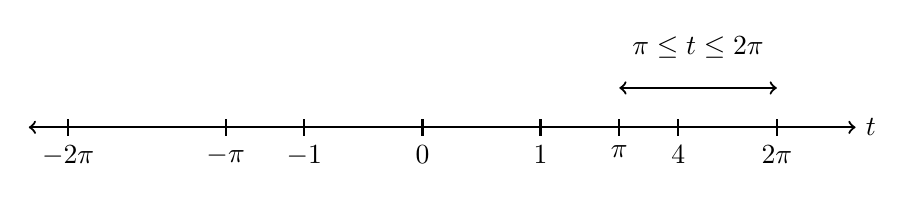
\begin{tikzpicture}

% Draw the line
\draw[thick, <->] (-5,0) -- (5.5,0) node[right] {$t$};

% Mark and label specific points
\foreach \x/\xtext in {-4.5/$-2\pi$, -2.5/$-\pi$, -1.5/$-1$, 0/$0$, 1.5/$1$, 2.5/$\pi$, 4.5/$2\pi$}
  \draw[thick] (\x,3pt) -- (\x,-3pt) node[below] {\xtext};

% Mark the point 4
\draw[thick] (3.25,3pt) -- (3.25,-3pt) node[below] {$4$};

% Draw the interval of continuity
\draw[thick,<->] (2.5,0.5) -- (4.5,0.5);
\node at (3.5,0.75) [above] {$\pi \leq t \leq 2\pi$};

\end{tikzpicture}
\end{center}


\section*{I.3: Separable Equation}

A first-order ordinary differential equation (ODE) is \textbf{separable} if it can be written in the form:

\[
y' = f(t)g(y)
\]

\textbf{Example:}

Consider the differential equation:

\[
y' = 2ty^2 + 3t^2y^2
\]

We can factor this as:

\[
y' = (2t + 3t^2)y^2
\]

Here, we have:

\[
f(t) = 2t + 3t^2, \quad g(y) = y^2
\]

An ODE of the form \( y' = g(y) \) is called \textbf{autonomous}.

A solution is called \textbf{stationary} if it is constant. If \( y = C \) is a stationary solution, then:

\[
y' = 0 \Rightarrow \boxed{0 = g(C)}
\]

\textbf{Example:}

Consider the equation:

\[
y' = 4y - y^3
\]

To find the stationary solutions, set:

\[
4y - y^3 = 0 \Rightarrow y(4 - y^2) = 0 \Rightarrow y(2 - y)(2 + y) = 0
\]

Thus, the stationary solutions are:

\[
y = 0, \quad y = 2, \quad y = -2
\]




\section*{Non-Stationary Solutions}

To find non-stationary solutions of the equation \( y' = g(y) \), we proceed as follows:

\[
y' = g(y) \quad \Rightarrow \quad \frac{1}{g(y)} y' = 1 
\]

Taking the integral on both sides:

\[
\int \frac{1}{g(y)} y' \, dt = \int 1 \, dt
\]

This simplifies to:

\[
\int \frac{1}{g(y)} \, dy = t + C
\]

The result is an implicit equation for our solution.

\textbf{Why can we divide by \( g(y) \)?}  
\( g(y) = 0 \) corresponds to stationary solutions, and we are looking for non-stationary solutions, i.e., \( g(y) \neq 0 \).

\section*{Example: Find All Solutions to \( y' = y^2 \)}

\textbf{Stationary Solutions:}  
Set \( y^2 = 0 \), which implies \( y = 0 \).

\textbf{Non-Stationary Solutions:}

Starting with the equation:

\[
\frac{1}{y^2} y' = 1
\]

Integrate both sides:

\[
\int \frac{1}{y^2} y' \, dt = \int 1 \, dt
\]

This simplifies to:

\[
\int \frac{1}{y^2} \, dy = t + C
\]

Evaluating the integral:

\[
-\frac{1}{y} = t + C
\]

We can find an explicit solution:

\[
-y = \frac{1}{t + C} \quad \Rightarrow \quad y = -\frac{1}{t + C}
\]



Each solution \( y = -\frac{1}{t + C} \) actually represents two solutions, one defined on \( (-\infty, -C) \) and the other on \( (-C, \infty) \).

\textbf{Note:} Our solution is discontinuous even though all functions in the original equation \( y' = y^2 \) are continuous.

\section*{General Separable Equations}

Consider the general separable equation:

\[
y' = f(t)g(y)
\]

If \( g(c) = 0 \), then \( y = c \) is a stationary solution (so set g(y) = 0).

For non-stationary solutions:

\[
\frac{1}{g(y)} y' = f(t)
\]

Taking the integral on both sides:

\[
\int \frac{1}{g(y)} y' \, dt = \int f(t) \, dt
\]

This simplifies to:

\[
\int \frac{1}{g(y)} \, dy = F(t) + C
\]

\section*{Example: Find All Solutions to \( \frac{dz}{dx} = \frac{3x + xz^2}{z + x^2z} \)}

First, rewrite the equation:

\[
\frac{dz}{dx} = \frac{x}{1 + x^2} \cdot \frac{3 + z^2}{z}
\]

Thus, we identify:

\[
f(x) = \frac{x}{1 + x^2}, \quad g(z) = \frac{3 + z^2}{z}
\]

\textbf{Stationary Solutions:}  
Set \( g(z) = 0 \):

\[
\frac{3 + z^2}{z} = 0 \quad \Rightarrow \quad 3 + z^2 = 0
\]

This equation has no real solution, so there are no stationary solutions.

\textbf{Non-Stationary Solutions:}

Start with:

\[
\frac{1}{g(z)} \frac{dz}{dx} = f(x)
\]

Which simplifies to:

\[
\frac{z}{3 + z^2} \cdot \frac{dz}{dx} = \frac{x}{1 + x^2}
\]

Integrate both sides:

\[
\int \frac{z}{3 + z^2} \frac{dz}{dx} \, dx = \int \frac{x}{1 + x^2} \, dx
\]

Use substitution:

- Let \( u = 3 + z^2 \), then \( du = 2z \, dz \).
- Let \( v = 1 + x^2 \), then \( dv = 2x \, dx \).

The integrals become:

\[
\int \frac{1}{2u} du = \int \frac{1}{2v} dv
\]

This integrates to:

\[
\frac{1}{2} \ln|u| = \frac{1}{2} \ln|v| + C
\]

Substituting back \( u \) and \( v \):

\[
\frac{1}{2} \ln|3 + z^2| = \frac{1}{2} \ln|1 + x^2| + C
\]



\section*{Initial Value Problems (IVPs)}

\textbf{Example:} Solve the initial value problem:

\[
y' = ty^2 - ty, \quad y(1) = 2
\]

We can factor the equation as:

\[
y' = t(y^2 - y)
\]

\textbf{Stationary Solutions:}  
Set \( y^2 - y = 0 \):

\[
y(y - 1) = 0 \quad \Rightarrow \quad y = 0 \quad \text{or} \quad y = 1
\]

Neither \( y = 0 \) nor \( y = 1 \) satisfies the initial condition \( y(1) = 2 \).

\begin{center}
\begin{tikzpicture}
    \draw[thick,->] (-1,0) -- (3,0) node[right] {$t$};
    \draw[thick,->] (0,-1) -- (0,3) node[above] {$y$};
    
    \draw[blue,thick] (-1,1) -- (3,1) node[below right] {$y=1$};
    \draw[red,thick] (-1,0) -- (3,0) node[below right] {$y=0$};

    \node at (1,2) [circle,fill,inner sep=1.5pt,label=above:{$(1,2)$}] {};
\end{tikzpicture}
\end{center}

As shown in the graph, neither \( y = 0 \) nor \( y = 1 \) passes through the point \( (1, 2) \).

\textbf{Other Solutions:}  
We solve the differential equation for non-stationary solutions:

\[
\frac{1}{y^2 - y} \frac{dy}{dt} = t \quad \Rightarrow \quad \frac{1}{y^2 - y} \, dy = t \, dt
\]

Integrate both sides:

\[
\int \frac{1}{y^2 - y} \, dy = \int t \, dt
\]

Using partial fractions:

\[
\frac{1}{y(y-1)} = \frac{A}{y} + \frac{B}{y-1}
\]

This leads to:

\[
1 = A(y - 1) + B(y) 
\]

By guessing \( A = -1 \) and \( B = 1 \), we get:

\[
\int \left( -\frac{1}{y} + \frac{1}{y-1} \right) dy = \int t \, dt
\]

Integrating both sides:

\[
-\ln|y| + \ln|y - 1| = \frac{t^2}{2} + C
\]

Using the logarithm property \( \ln(a) - \ln(b) = \ln\left(\frac{a}{b}\right) \), this simplifies to:

\[
\ln\left|\frac{y - 1}{y}\right| = \frac{t^2}{2} + C
\]

\textbf{Applying the Initial Condition:}  
Given \( y(1) = 2 \):

\[
\ln\left|\frac{2 - 1}{2}\right| = \frac{1^2}{2} + C
\]

\[
\ln\left(\frac{1}{2}\right) = \frac{1}{2} + C \quad \Rightarrow \quad C = \ln\left(\frac{1}{2}\right) - \frac{1}{2}
\]

Substituting \( C \) back into the equation:

\[
\ln\left|\frac{y - 1}{y}\right| = \frac{t^2}{2} + \ln\left(\frac{1}{2}\right) - \frac{1}{2}
\]




\section*{Uniqueness and Existence Theorem}

If \( f(t) \) is continuous on \( (a, b) \) and \( g(y) \) is continuous and differentiable on \( (c, d) \), then for every \( t_I \in (a, b) \) and \( y_I \in (c, d) \), there exists a unique continuous solution to the equation

\[
y' = f(t)g(y)
\]

with the initial condition \( y(t_I) = y_I \), defined on some interval around \( t_I \). The solution is determined by our method.

\section*{Example}

Consider the differential equation:

\[
\frac{dy}{dt} = 3y^{2/3}, \quad y(0) = 0
\]

\textbf{Stationary Solution:}  
\( y = 0 \) is a stationary solution, and it solves our initial value problem (IVP).

However, \( g(y) = 3y^{2/3} \) is not differentiable at \( y = 0 \), so we might have other solutions.

\textbf{Finding Other Solutions:}

\[
\frac{1}{3y^{2/3}} \frac{dy}{dt} = 1
\]

Integrating both sides:

\[
\int \frac{1}{3y^{2/3}} \, dy = \int 1 \, dt
\]

This simplifies to:

\[
y^{1/3} = t + C
\]

Raising both sides to the power of 3:

\[
y = (t + C)^3
\]

\textbf{Applying the Initial Condition:}  
For \( y(0) = 0 \), we get \( C = 0 \), so:

\[
y = t^3
\]

Thus, \( y = t^3 \) also solves our IVP.


\section*{Lecture 3, Tuesday 9/3/2024}


\textbf{Quiz tomorrow:} Up to Section I.3

\section*{I.4. Theory}

Consider Initial Value Problems (IVPs) of the form:
\[
y' = f(t,y), \quad y(t_i) = y_i
\]

We say the problem is \textit{well-posed} if:

\begin{enumerate}
    \item There exists a solution
    \item The solution is unique
    \item The solution depends continuously on the initial conditions
\end{enumerate}

\subsection*{Existence and Uniqueness}

Consider a set $S$ of points in the $(t,y)$ plane.

\begin{figure}[h]
    \centering
    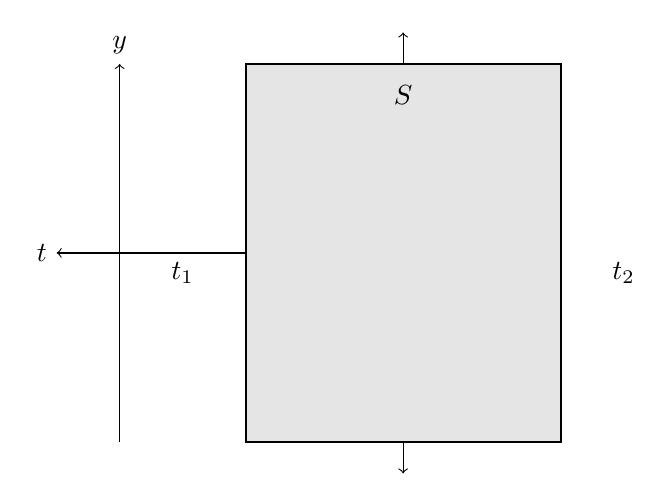
\begin{tikzpicture}[scale=0.8]
        % Draw the axes
        \draw[->] (6,0) -- (-1,0) node[left] {$t$};
        \draw[->] (0,-3) -- (0,3) node[above] {$y$};
        
        % Draw the vertical rectangle S
        \fill[gray!20] (2,-3) rectangle (7,3);
        \draw[thick] (2,-3) rectangle (7,3);
        
        % Label the set S
        \node at (4.5,2.5) {$S$};
        
        % Label the t-coordinates
        \node[below] at (1,0) {$t_1$};
        \node[below] at (8,0) {$t_2$};
        
        % Add arrows to indicate infinite extension in y-direction
        \draw[->] (4.5,3) -- (4.5,3.5);
        \draw[->] (4.5,-3) -- (4.5,-3.5);
    \end{tikzpicture}
    \caption{The set $S$ in the $(t,y)$ plane}
    \label{fig:set_S}
\end{figure}

If $f(t,y)$ is continuous on $S$ and $\frac{\partial f}{\partial y}$ is continuous on $S$, then for any $(t_i, y_i) \in S$, there exists a unique continuous solution $Y(t)$ to the initial value problem:
\[
\begin{cases}
y' = f(t,y) \\
Y(t_i) = y_i
\end{cases}
\]
defined over some interval $(a,b)$ containing $t_i$.

Moreover, the interval $(a,b)$ can be extended as long as $(t, Y(t))$ remains inside $S$.

\textbf{Example:} Consider $y' = \frac{\sin(t+ty^2)}{1+t^2}$, $y(0) = 1$

Let's show that there is a unique solution defined on $(-1, 1)$.

\textbf{Solution:} 
For $f(t, y) = \frac{\sin(t+ty^2)}{1+t^2}$, $f$ is continuous except at $t = \pm 1$.

$\frac{\partial f}{\partial y} = \frac{2ty\cos(t+ty^2)}{1+t^2}$, which is also continuous except at $t = \pm 1$.

By the Existence and Uniqueness Theorem, since $f$ and $\frac{\partial f}{\partial y}$ are continuous on $S$, there exists a unique solution $y(t)$ to the initial value problem, defined on some interval containing $t=0$. This interval can be extended as long as $(t,y(t))$ remains inside $S$, which in this case is the entire interval $(-1,1)$.

Since $t_i = 0$, $y_i = 1 \implies (0,1) \in S$, the theorem tells us we have a unique solution $Y(t)$ defined on a larger $(a, b)$ such that $y(t)$ remains inside $S$.

Since any solution will not leave $S$ as long as $-1 < t < 1$, we get $(a,b) = (-1, 1)$.

So, we choose $S$ as follows:

\begin{figure}[h]
    \centering
    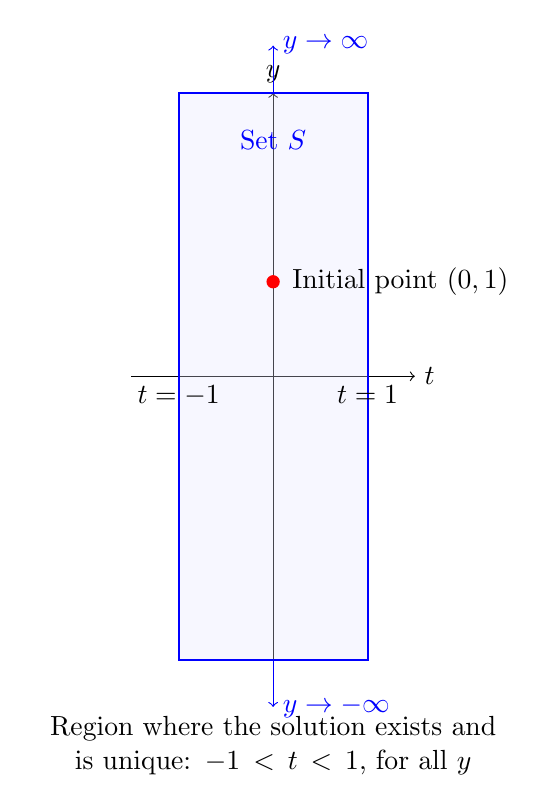
\begin{tikzpicture}[scale=1.2]
        % Draw the axes
        \draw[->] (-1.5,0) -- (1.5,0) node[right] {$t$};
        \draw[->] (0,-3) -- (0,3) node[above] {$y$};
        
        % Draw the vertical rectangle S with transparent fill
        \fill[blue!10, opacity=0.3] (-1,-3) rectangle (1,3);
        \draw[thick, blue] (-1,-3) rectangle (1,3);
        
        % Label the set S
        \node[blue] at (0,2.5) {Set $S$};
        
        % Label the t-coordinates
        \node[below] at (-1,0) {$t=-1$};
        \node[below] at (1,0) {$t=1$};
        
        % Add arrows and labels to indicate infinite extension in y-direction
        \draw[->, blue] (0,3) -- (0,3.5) node[right] {$y \to \infty$};
        \draw[->, blue] (0,-3) -- (0,-3.5) node[right] {$y \to -\infty$};
        
        % Mark the initial point (0,1)
        \fill[red] (0,1) circle (2pt);
        \node[right] at (0.1,1) {Initial point $(0,1)$};
        
        % Add explanation
        \node[text width=6cm, align=center, below] at (0,-3.5) 
        {Region where the solution exists and is unique: $-1 < t < 1$, for all $y$};
    \end{tikzpicture}
    \caption{Set $S$ where the solution to the differential equation is guaranteed to exist and be unique}
    \label{fig:set_S_example}
\end{figure}

\pagebreak

\textbf{Example:} Consider the differential equation $y' = \frac{1}{t^2 + y^2 - 1}$, with initial condition $y(0) = 0$. Find the set $S$ where the solution is guaranteed to exist and be unique.

\textbf{Solution:} 
The function $f(t,y) = \frac{1}{t^2 + y^2 - 1}$ is discontinuous when $t^2 + y^2 = 1$. This equation describes a circle with radius 1 centered at the origin.

The set $S$ where the solution exists and is unique should be the interior of this circle, excluding the circle itself. We can represent this as:

\[S = \{(t,y) : t^2 + y^2 < 1\}\]

Let's visualize this set:

\begin{figure}[h]
    \centering
    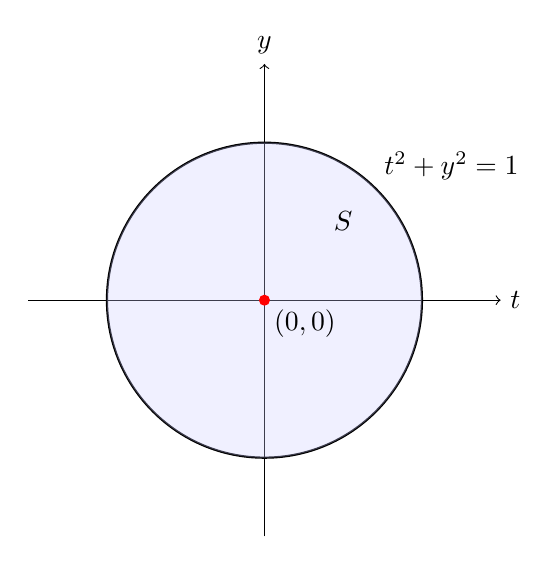
\begin{tikzpicture}[scale=2]
        % Draw the axes
        \draw[->] (-1.5,0) -- (1.5,0) node[right] {$t$};
        \draw[->] (0,-1.5) -- (0,1.5) node[above] {$y$};
        
        % Draw the circle t^2 + y^2 = 1
        \draw[thick] (0,0) circle (1);
        
        % Fill the interior of the circle (set S) with transparent highlight
        \fill[blue!20, opacity=0.3] (0,0) circle (1);
        
        % Label the set S
        \node at (0.5,0.5) {$S$};
        
        % Mark the initial point (0,0)
        \fill[red] (0,0) circle (1pt);
        \node[below right] at (0,0) {$(0,0)$};
        
        % Label the circle
        \node[above right] at (0.7,0.7) {$t^2 + y^2 = 1$};
    \end{tikzpicture}
    \caption{Set $S$ for the given differential equation}
    \label{fig:set_S_circle_example}
\end{figure}

The solution is guaranteed to exist and be unique within this circular region $S$, but not on or outside the boundary where $t^2 + y^2 = 1$.

\textbf{Example:} Consider the differential equation $y' = \frac{1}{t^2 + y^2 - 1}$, with initial condition $y(0) = 3$. Let's visualize the set $S$ where the solution is guaranteed to exist and be unique.

\textbf{Solution:} 
The function $f(t,y) = \frac{1}{t^2 + y^2 - 1}$ is discontinuous when $t^2 + y^2 = 1$. This equation describes a circle with radius 1 centered at the origin.

The set $S$ where the solution exists and is unique should be the region outside this circle, including the initial point $(0,3)$. We can represent this as:

\[S = \{(t,y) : t^2 + y^2 > 1\}\]

Let's visualize this set:

\pagebreak
\begin{figure}[h]
    \centering
    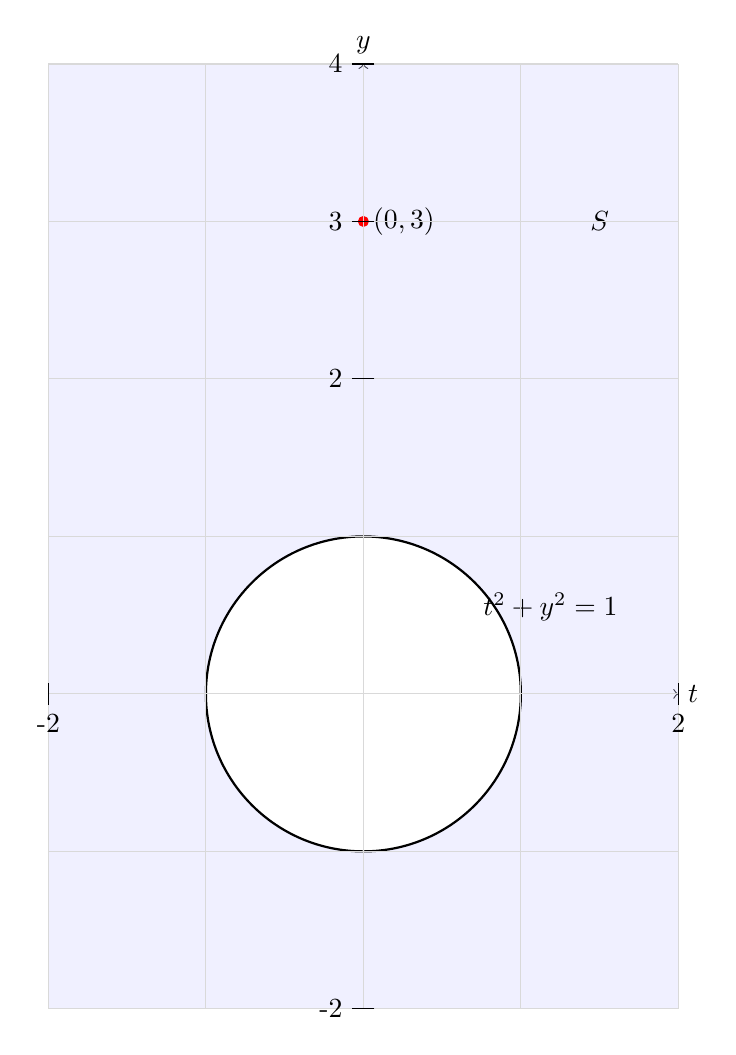
\begin{tikzpicture}[scale=2]
        % Draw the axes
        \draw[->] (-2,0) -- (2,0) node[right] {$t$};
        \draw[->] (0,-2) -- (0,4) node[above] {$y$};
        
        % Fill the exterior of the circle (set S) with transparent highlight
        \begin{scope}
            \clip (-2,-2) rectangle (2,4);
            \fill[blue!20, opacity=0.3] (-2,-2) rectangle (2,4);
            \fill[white] (0,0) circle (1);
        \end{scope}
        
        % Draw the circle t^2 + y^2 = 1
        \draw[thick] (0,0) circle (1);
        \node[anchor=north west] at (0.7,0.7) {$t^2 + y^2 = 1$};
        
        % Label the set S
        \node at (1.5,3) {$S$};
        
        % Mark the initial point (0,3)
        \fill[red] (0,3) circle (1pt);
        \node[right] at (0,3) {$(0,3)$};
        
        % Add grid lines for better visualization
        \draw[gray!30, step=1] (-2,-2) grid (2,4);
        
        % Label the axes
        \foreach \x in {-2,2}
            \draw (\x,2pt) -- (\x,-2pt) node[below] {\x};
        \foreach \y in {-2,2,3,4}
            \draw (2pt,\y) -- (-2pt,\y) node[left] {\y};
    \end{tikzpicture}
    \caption{Set $S$ for the given differential equation with $y(0) = 3$}
    \label{fig:set_S_circle_example_y0_3}
\end{figure}

The solution is guaranteed to exist and be unique within the region $S$, which is the area outside the circle $t^2 + y^2 = 1$, including the initial point $(0,3)$.


\pagebreak

\section{I.5 - Graphical Methods}

\subsection{Phase Portraits for Autonomous Equations}

Consider the autonomous differential equation:

\[
\frac{dy}{dt} = g(y)
\]

Our goal is to describe the qualitative behavior of solutions without explicitly solving the equation.

\begin{itemize}
    \item When $g(y) = 0$:
        \begin{itemize}
            \item $y' = 0$
            \item We have a stationary solution
        \end{itemize}
    
    \item When $g(y) > 0$:
        \begin{itemize}
            \item $y' > 0$
            \item The solution is increasing
        \end{itemize}
    
    \item When $g(y) < 0$:
        \begin{itemize}
            \item $y' < 0$
            \item The solution is decreasing
        \end{itemize}
\end{itemize}


\subsection*{Example: $y' = 4y - y^3$}

Let's analyze the differential equation $y' = 4y - y^3$.

\begin{enumerate}
    \item First, we find the stationary solutions:
    \[
    4y - y^3 = y(4 - y^2) = y(2-y)(2+y) = 0
    \]
    Thus, the stationary solutions are $y = 0, \pm 2$.

    \item Next, we determine the sign of $g(y) = 4y - y^3$ between these zeros:
    \begin{align*}
        g(1) &= 4(1) - (1)^3 = 3 > 0 \\
        g(3) &= 4(3) - (3)^3 = 12 - 27 = -15 < 0 \\
        g(-3) &= 4(-3) - (-3)^3 = -12 + 27 = 15 > 0 \\
        g(-1) &= 4(-1) - (-1)^3 = -4 + 1 = -3 < 0
    \end{align*}
\end{enumerate}

Based on this analysis, we can create a phase portrait:

\begin{figure}[h]
    \centering
    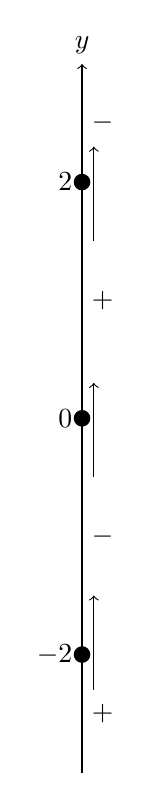
\begin{tikzpicture}[scale=1.5]
        % Draw y-axis
        \draw[->] (0,-3) -- (0,3) node[above] {$y$};
        
        % Plot points and labels
        \foreach \y/\label in {2/2, 0/0, -2/-2} {
            \fill (0,\y) circle (2pt);
            \node[left] at (0,\y) {$\y$};
        }
        
        % Add + and - signs
        \node[right] at (0,2.5) {$-$};
        \node[right] at (0,1) {$+$};
        \node[right] at (0,-1) {$-$};
        \node[right] at (0,-2.5) {$+$};
        
        % Add arrows to show direction
        \draw[->] (0.1,1.5) -- (0.1,2.3);
        \draw[->] (0.1,-0.5) -- (0.1,0.3);
        \draw[->] (0.1,-2.3) -- (0.1,-1.5);
    \end{tikzpicture}
    \caption{Phase portrait for $y' = 4y - y^3$}
    \label{fig:phase_portrait_4y_minus_y3}
\end{figure}

The phase portrait shows:
\begin{itemize}
    \item Solutions increase when $y \in (-\infty, -2) \cup (0, 2)$
    \item Solutions decrease when $y \in (-2, 0) \cup (2, \infty)$
    \item Stationary solutions at $y = 0, \pm 2$
\end{itemize}




This diagram is called a phase portrait or phase line. It provides valuable information about the behavior of solutions $y(t)$ for different initial conditions:

\begin{itemize}
    \item For $y(t)$ starting in $(-\infty, -2)$:
        \begin{itemize}
            \item $y(t)$ increases as $t$ increases
            \item $y(t) \rightarrow -2$ as $t \rightarrow \infty$ (asymptotically approaching -2)
        \end{itemize}
    
    \item For $y(t)$ starting in $(-2, 0)$:
        \begin{itemize}
            \item $y(t)$ is decreasing
            \item $y(t) \rightarrow -2$ as $t \rightarrow \infty$
        \end{itemize}
    
    \item For $y(t)$ starting in $(0, 2)$:
        \begin{itemize}
            \item $y(t)$ is increasing
            \item $y(t) \rightarrow 2$ as $t \rightarrow \infty$ (asymptotically approaching 2)
        \end{itemize}
    
    \item For $y(t)$ starting in $(2, \infty)$:
        \begin{itemize}
            \item $y(t)$ is decreasing
            \item $y(t) \rightarrow 2$ as $t \rightarrow \infty$ (asymptotically approaching 2)
        \end{itemize}
\end{itemize}


Sketch solutions:

\begin{figure}[h]
    \centering
    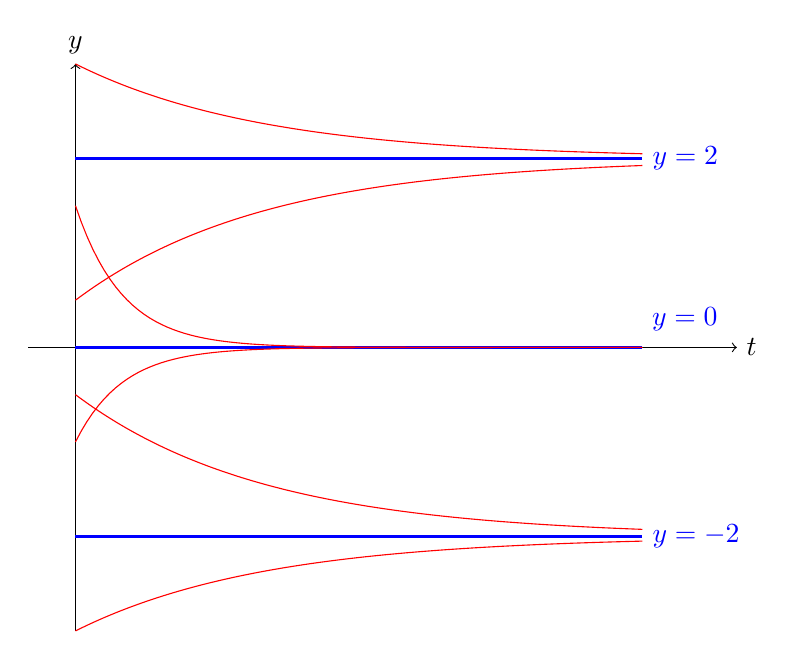
\begin{tikzpicture}[scale=1.2]
        % Axes
        \draw[->] (-0.5,0) -- (7,0) node[right] {$t$};
        \draw[->] (0,-3) -- (0,3) node[above] {$y$};
        
        % Constant solutions
        \draw[thick, blue] (0,2) -- (6,2) node[right] {$y=2$};
        \draw[thick, blue] (0,0) -- (6,0) node[right] {};
        \draw[thick, blue] (0,-2) -- (6,-2) node[right] {$y=-2$};

        % Label for y=0
        \node[right, blue] at (6,0.3) {$y=0$};
        
        % Solutions approaching -2
        \draw[red] plot[domain=0:6, samples=100] (\x, {-2+1.5*exp(-\x/2)});
        \draw[red] plot[domain=0:6, samples=100] (\x, {-2-exp(-\x/2)});
        
        % Solutions approaching 2
        \draw[red] plot[domain=0:6, samples=100] (\x, {2-1.5*exp(-\x/2)});
        \draw[red] plot[domain=0:6, samples=100] (\x, {2+exp(-\x/2)});
        
        % Solution approaching 0
        \draw[red] plot[domain=0:6, samples=100] (\x, {1.5*exp(-2*\x)});
        \draw[red] plot[domain=0:6, samples=100] (\x, {-exp(-2*\x)});
    \end{tikzpicture}
    \caption{Sketch of solutions for $y' = 4y - y^3$}
    \label{fig:solutions_4y_minus_y3}
\end{figure}

This figure illustrates:
\begin{itemize}
    \item Constant solutions at $y=2$, $y=0$, and $y=-2$ (blue lines)
    \item Solutions approaching $y=2$ from above and below
    \item Solutions approaching $y=-2$ from above and below
    \item Solutions approaching $y=0$ from above and below
\end{itemize}

The red curves represent various solutions to the differential equation, showing how they behave over time depending on their initial conditions.

We classify stationary solutions as follows:

\begin{itemize}
    \item \textbf{Stable or attracting:} All nearby solutions move towards it as $t \rightarrow \infty$. 
          \\ (In this case: $y = \pm 2$)
    
    \item \textbf{Unstable or repelling:} All nearby solutions move away from it as $t \rightarrow \infty$. 
          \\ (In this case: $y = 0$)
    
    \item \textbf{Semi-stable:} Some solutions move towards it and some move away from it as $t \rightarrow \infty$.
\end{itemize}

\begin{figure}[h]
    \centering
    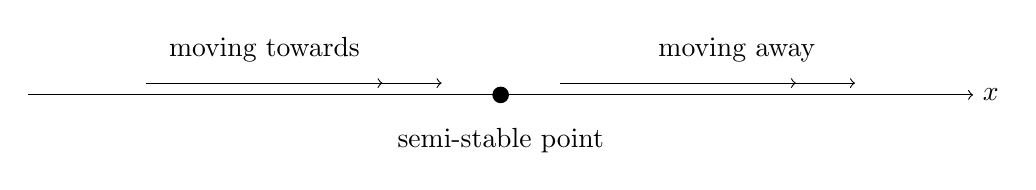
\begin{tikzpicture}[scale=1.5]
        % Draw the x-axis
        \draw[->] (-4,0) -- (4,0) node[right] {$x$};
        
        % Draw the semi-stable point
        \fill[black] (0,0) circle (2pt);
        \node[below] at (0,-0.2) {semi-stable point};
        
        % Draw arrows moving towards the point
        \draw[->] (-3,0.1) -- (-1,0.1);
        \draw[->] (-2.5,0.1) -- (-0.5,0.1);
        
        % Draw arrows moving away from the point
        \draw[->] (1,0.1) -- (3,0.1);
        \draw[->] (0.5,0.1) -- (2.5,0.1);
        
        % Labels
        \node[above] at (-2,0.2) {moving towards};
        \node[above] at (2,0.2) {moving away};
    \end{tikzpicture}
    \caption{Behavior near a semi-stable point}
    \label{fig:semi_stable_point}
\end{figure}



\textbf{Example:} Consider the differential equation $y' = y^2$

\begin{itemize}
    \item Stationary solution: $y = 0$
    \item For $y \neq 0$: $y^2 > 0$, implying solutions move away from $y = 0$
\end{itemize}

This example demonstrates an unstable stationary solution at $y = 0$.

\begin{figure}[h]
    \centering
    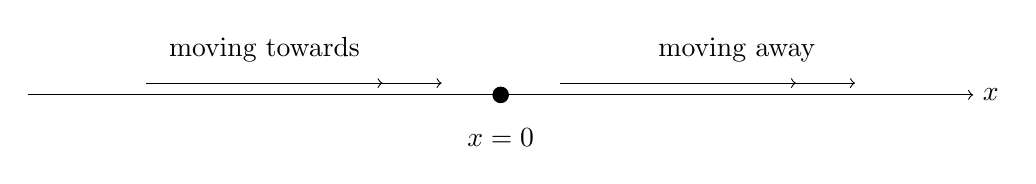
\begin{tikzpicture}[scale=1.5]
        % Draw the x-axis
        \draw[->] (-4,0) -- (4,0) node[right] {$x$};
        
        % Draw arrows moving towards the origin
        \draw[->] (-3,0.1) -- (-1,0.1);
        \draw[->] (-2.5,0.1) -- (-0.5,0.1);
        
        % Draw arrows moving away from the origin
        \draw[->] (1,0.1) -- (3,0.1);
        \draw[->] (0.5,0.1) -- (2.5,0.1);
        
        % Labels
        \node[above] at (-2,0.2) {moving towards};
        \node[above] at (2,0.2) {moving away};
        
        % Origin point
        \fill[black] (0,0) circle (2pt);
        \node[below] at (0,-0.2) {$x=0$};
    \end{tikzpicture}
    \caption{Behavior on x-axis for $y'=y^2$}
    \label{fig:x_axis_behavior}
\end{figure}

\begin{figure}[h]
    \centering
    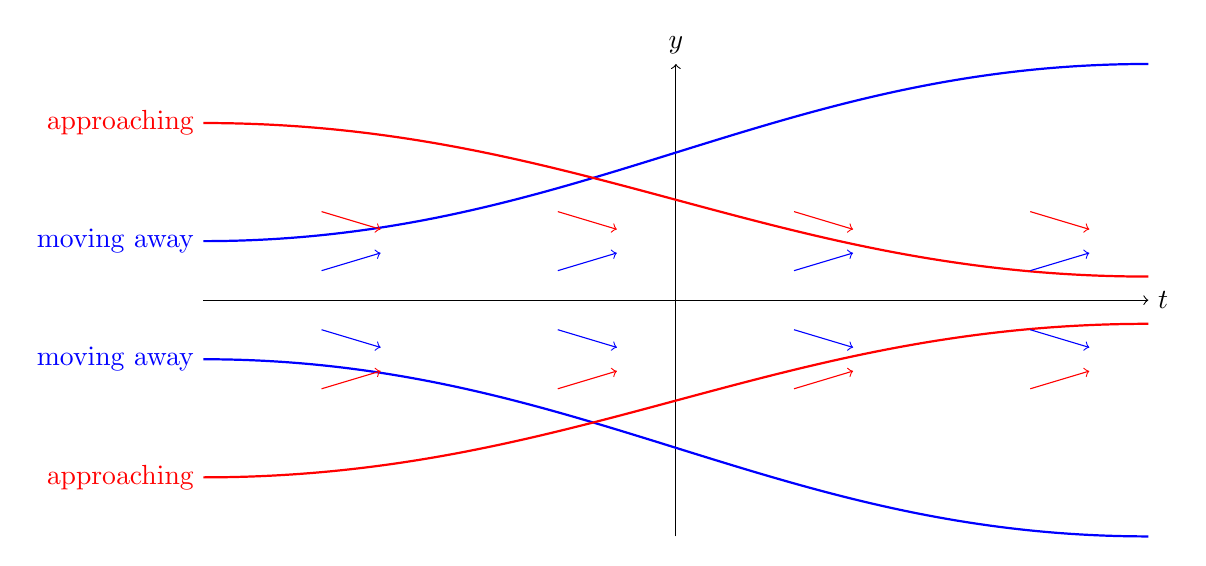
\begin{tikzpicture}[scale=1.5]
        % Draw the axes
        \draw[->] (-4,0) -- (4,0) node[right] {$t$};
        \draw[->] (0,-2) -- (0,2) node[above] {$y$};
        
        % Draw the y=0 line
        \draw[dashed] (-4,0) -- (4,0);
        
        % Draw solutions moving away from y=0
        \draw[blue, thick] (-4,0.5) to[out=0,in=180] (4,2);
        \draw[blue, thick] (-4,-0.5) to[out=0,in=180] (4,-2);
        
        % Draw solutions approaching y=0
        \draw[red, thick] (-4,1.5) to[out=0,in=180] (4,0.2);
        \draw[red, thick] (-4,-1.5) to[out=0,in=180] (4,-0.2);
        
        % Labels
        \node[blue, left] at (-4,0.5) {moving away};
        \node[blue, left] at (-4,-0.5) {moving away};
        \node[red, left] at (-4,1.5) {approaching};
        \node[red, left] at (-4,-1.5) {approaching};
        
        % Arrows indicating direction
        \foreach \x in {-3,-1,1,3} {
            \draw[->, blue] (\x,0.25) -- (\x+0.5,0.4);
            \draw[->, blue] (\x,-0.25) -- (\x+0.5,-0.4);
            \draw[->, red] (\x,0.75) -- (\x+0.5,0.6);
            \draw[->, red] (\x,-0.75) -- (\x+0.5,-0.6);
        }
    \end{tikzpicture}
    \caption{Behavior of solutions in t-y plane for $y'=y^2$}
    \label{fig:ty_plane_behavior}
\end{figure}

This figure illustrates the behavior of solutions to $y'=y^2$ near the stationary solution $y=0$. The blue curves represent solutions moving away from $y=0$, while the red curves represent solutions approaching $y=0$. 
This demonstrates that $y=0$ is an unstable or repelling stationary solution.



For stability think of a pendulum


\begin{figure}[h]
    \centering
    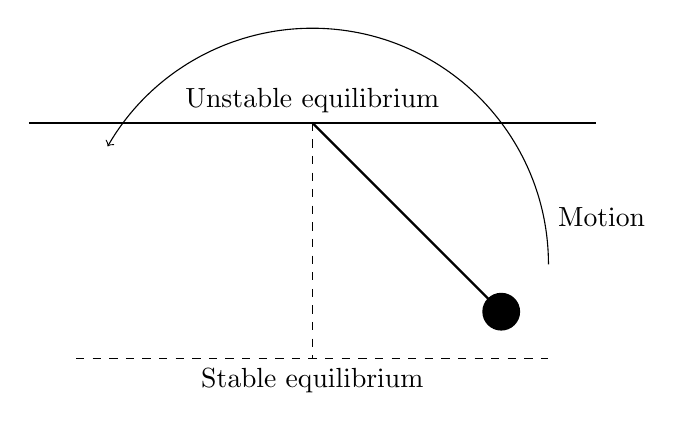
\begin{tikzpicture}[scale=1.2]
        % Draw the support
        \draw[thick] (-3,3) -- (3,3);
        
        % Draw the pendulum rod
        \draw[thick] (0,3) -- (2,1);
        
        % Draw the pendulum bob
        \fill[black] (2,1) circle (0.2);
        
        % Draw the arc to show motion
        \draw[->] (2.5,1.5) arc (0:150:2.5);
        
        % Label the stationary points
        \node[above] at (0,3) {Unstable equilibrium};
        \node[below] at (0,0.5) {Stable equilibrium};
        
        % Draw dashed lines to show equilibrium positions
        \draw[dashed] (0,3) -- (0,0.5);
        \draw[dashed] (-2.5,0.5) -- (2.5,0.5);
        
        % Label the motion
        \node[right] at (2.5,2) {Motion};
        
    \end{tikzpicture}
    \caption{Pendulum illustrating stable and unstable equilibrium points}
    \label{fig:pendulum}
\end{figure}

This figure illustrates a pendulum moving from right to left. The top position (vertically upright) represents an unstable equilibrium, while the bottom position represents a stable equilibrium. These correspond to the stationary solutions of the pendulum's differential equation.


unstable solution is pendulum at the top and stable is pendulum at the bottom





\subsection*{Example: Phase Line Analysis}

Consider the differential equation:

\[
y' = \frac{(y^2-1)(y-3)^2}{(y+3)^2}
\]

\textbf{Stationary Solutions:}
\begin{itemize}
    \item $y = -1$
    \item $y = 1$
    \item $y = 3$
\end{itemize}

\textbf{Note:} $y = -3$ is undefined in the equation.

We will now draw the phase line for this differential equation to analyze its behavior.

\begin{figure}[h]
    \centering
    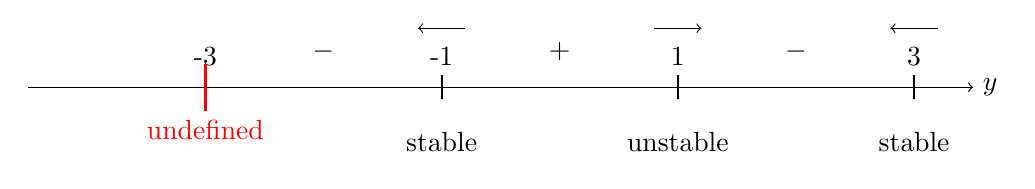
\begin{tikzpicture}[scale=1.5]
        % Draw the y-axis
        \draw[->] (-0.5,0) -- (7.5,0) node[right] {$y$};
        
        % Mark and label the points
        \foreach \x/\xtext in {1/-3, 3/-1, 5/1, 7/3}
            \draw[thick] (\x,-0.1) -- (\x,0.1) node[above] {\xtext};
        
        % Show the undefined point at y = -3
        \draw[red, thick] (1,-0.2) -- (1,0.2);
        \node[below, red] at (1,-0.2) {undefined};
        
        % Add + and - signs between points
        \node at (2,0.3) {$-$};
        \node at (4,0.3) {$+$};
        \node at (6,0.3) {$-$};
        
        % Add arrows to show stability
        \draw[->] (3.2,0.5) -- (2.8,0.5);
        \draw[->] (4.8,0.5) -- (5.2,0.5);
        \draw[<-] (6.8,0.5) -- (7.2,0.5);
        
        % Label stationary solutions
        \node[below] at (3,-0.3) {stable};
        \node[below] at (5,-0.3) {unstable};
        \node[below] at (7,-0.3) {stable};
    \end{tikzpicture}
    \caption{Phase line for $y' = (y^2-1)(y-3)^2 / (y+3)^2$}
    \label{fig:phase_line}
\end{figure}




Note: stability only applies to stationary solutions, not to undefined points.

Sketch
\begin{figure}[h]
    \centering
    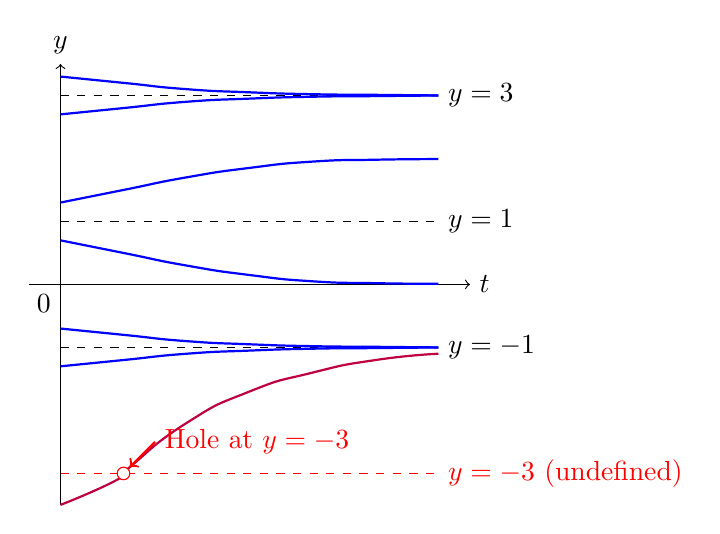
\begin{tikzpicture}[scale=0.8]
        % Draw the axes
        \draw[->] (-0.5,0) -- (6.5,0) node[right] {$t$};
        \draw[->] (0,-3.5) -- (0,3.5) node[above] {$y$};
        
        % Draw the horizontal lines for y = 3, 1, -1, -3
        \draw[dashed] (0,3) -- (6,3) node[right] {$y=3$};
        \draw[dashed] (0,1) -- (6,1) node[right] {$y=1$};
        \draw[dashed] (0,-1) -- (6,-1) node[right] {$y=-1$};
        \draw[dashed, red] (0,-3) -- (6,-3) node[right, red] {$y=-3$ (undefined)};
        
        % Draw some solution curves
        \draw[thick, blue] plot [smooth, tension=1] coordinates {(0,3.3) (1,3.2) (2,3.1) (3,3.05) (4,3.02) (5,3.01) (6,3)};
        \draw[thick, blue] plot [smooth, tension=1] coordinates {(0,2.7) (1,2.8) (2,2.9) (3,2.95) (4,2.98) (5,2.99) (6,3)};
        \draw[thick, blue] plot [smooth, tension=1] coordinates {(0,1.3) (1,1.5) (2,1.7) (3,1.85) (4,1.95) (5,1.98) (6,1.99)};
        \draw[thick, blue] plot [smooth, tension=1] coordinates {(0,0.7) (1,0.5) (2,0.3) (3,0.15) (4,0.05) (5,0.02) (6,0.01)};
        \draw[thick, blue] plot [smooth, tension=1] coordinates {(0,-0.7) (1,-0.8) (2,-0.9) (3,-0.95) (4,-0.98) (5,-0.99) (6,-1)};
        \draw[thick, blue] plot [smooth, tension=1] coordinates {(0,-1.3) (1,-1.2) (2,-1.1) (3,-1.05) (4,-1.02) (5,-1.01) (6,-1)};
        
        % Draw a line crossing y = -3 and approaching y = -1
        \draw[thick, purple] plot [smooth, tension=1] coordinates {(0,-3.5) (0.9,-3.1) (1.1,-2.9) (2,-2.2) (3,-1.7) (4,-1.4) (5,-1.2) (6,-1.1)};
       
        % Add a clear hole at y = -3
        \fill[white] (1,-3) circle (0.1);
        \draw[red] (1,-3) circle (0.1);
        
        % Add an arrow pointing to the hole
        \draw[->, red, thick] (1.5,-2.5) -- (1.1,-2.9);
        \node[red, right] at (1.5,-2.5) {Hole at $y=-3$};
        
        % Label the axes
        \node[below left] at (0,0) {0};
        
    \end{tikzpicture}
    \caption{Sketch of solutions for $y' = (y^2-1)(y-3)^2 / (y+3)^2$, including a solution crossing $y=-3$ with a clear hole}
    \label{fig:solution_sketch}
\end{figure}




\textbf{Example:} Consider the differential equation $y' = t - y^2$

\textbf{Procedure:} To sketch the slope field:
\begin{enumerate}
    \item Choose a representative selection of $(t, y)$ points.
    \item At each point $(t,y)$, draw an arrow with slope $t - y^2$.
    \item Connect the arrows to visualize solution curves.
\end{enumerate}

\textbf{Sample calculations:}
\begin{align*}
    \text{At } (0,0):& \quad t - y^2 = 0 \\
    \text{At } (1,0):& \quad t - y^2 = 1 \\
    \text{At } (-1,0):& \quad t - y^2 = -1 \\
    \text{At } (0,\pm 1):& \quad t - y^2 = -1
\end{align*}

\pagebreak
Continue this process for other points to build a comprehensive slope field.

\begin{figure}[h!]
    \centering
    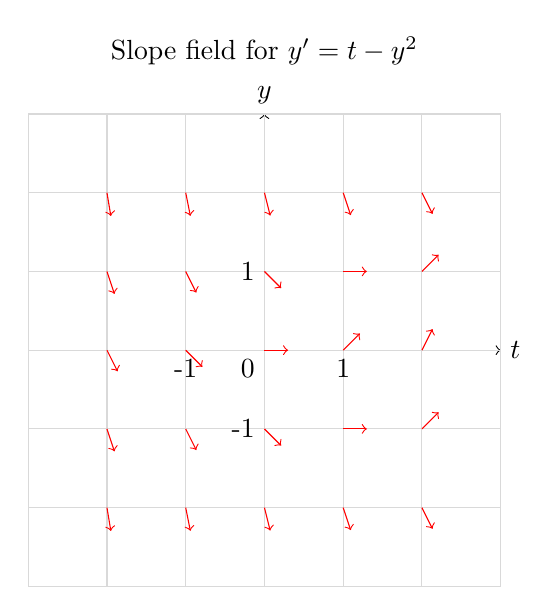
\begin{tikzpicture}[scale=1]
        % Draw the axes
        \draw[->] (-3,0) -- (3,0) node[right] {$t$};
        \draw[->] (0,-3) -- (0,3) node[above] {$y$};
        
        % Draw grid lines
        \draw[gray!30] (-3,-3) grid (3,3);
        
        % Draw arrows representing the slope field
        \foreach \x in {-2,-1,0,1,2} {
            \foreach \y in {-2,-1,0,1,2} {
                \pgfmathsetmacro{\slope}{\x - \y*\y}
                \draw[red,->] (\x,\y) -- ++({0.3*cos(atan(\slope))},{0.3*sin(atan(\slope))});
            }
        }
        
        % Label the axes
        \node[below left] at (0,0) {0};
        \node[below] at (1,0) {1};
        \node[below] at (-1,0) {-1};
        \node[left] at (0,1) {1};
        \node[left] at (0,-1) {-1};
        
        % Add title
        \node[above] at (0,3.5) {Slope field for $y' = t - y^2$};
    \end{tikzpicture}
    \caption{Slope field for the differential equation $y' = t - y^2$}
    \label{fig:slope_field}
\end{figure}

\vspace{-0.5cm}

If $y(0) = 1$, then the point should follow the slope field:

\begin{figure}[h!]
    \centering
    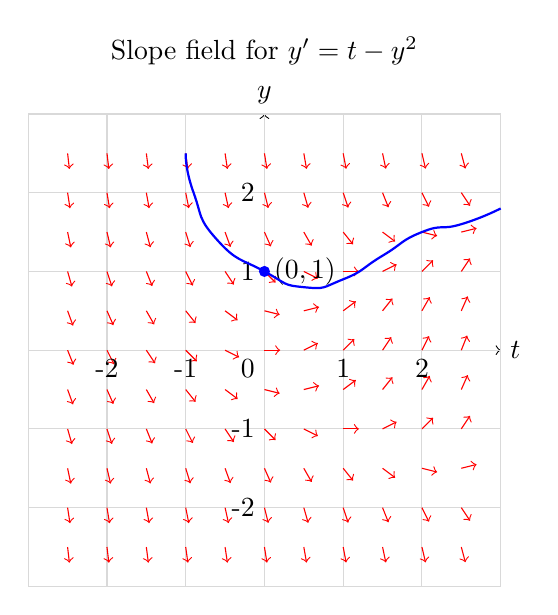
\begin{tikzpicture}[scale=1]
        % Draw the axes
        \draw[->] (-3,0) -- (3,0) node[right] {$t$};
        \draw[->] (0,-3) -- (0,3) node[above] {$y$};
        
        % Draw grid lines
        \draw[gray!30] (-3,-3) grid (3,3);
        
        % Draw arrows representing the slope field
        \foreach \x in {-2.5,-2,...,2.5} {
            \foreach \y in {-2.5,-2,...,2.5} {
                \pgfmathsetmacro{\slope}{\x - \y*\y}
                \draw[red,->] (\x,\y) -- ++({0.2*cos(atan(\slope))},{0.2*sin(atan(\slope))});
            }
        }
        
        % Label the axes
        \node[below left] at (0,0) {0};
        \foreach \x in {-2,-1,1,2} {
            \node[below] at (\x,0) {\x};
        }
        \foreach \y in {-2,-1,1,2} {
            \node[left] at (0,\y) {\y};
        }
        
        % Add title
        \node[above] at (0,3.5) {Slope field for $y' = t - y^2$};
        
        % Mark the initial point
        \fill[blue] (0,1) circle (2pt);
        \node[right] at (0,1) {$(0,1)$};
        
        % Draw the curve following the slope field (corrected direction)
        \draw[thick, blue] plot [smooth, tension=1] 
            coordinates {(-1,2.5) (-0.9,2) (-0.6,1.4) (0,1) (0.5,0.8) (1,0.9) (1.5,1.2) (2,1.5) (2.5,1.6) (3,1.8)};
    \end{tikzpicture}
    \caption{Slope field for $y' = t - y^2$ with initial point $y(0) = 1$ and solution curve}
    \label{fig:slope_field_with_solution_corrected}
\end{figure}
\pagebreak

\section*{Lecture 4, Thursday 9/5/2024}

\section{I.6 Applications of Differential Equations}

\subsection{I.6.1 Tanks and Mixtures}

\subsubsection{I.6.1.1 IRS Method: Identify, Reduce, Solve}

In tank and mixture problems, we often encounter scenarios where:

\begin{itemize}
    \item Water flows into and out of a tank
    \item Salt is mixed into the water
    \item The concentration of salt varies over time
    \item The mixture in the tank is continuously leaving
\end{itemize}

Our primary interest is in understanding how the salt content changes over time.

\begin{figure}[h]
    \centering
    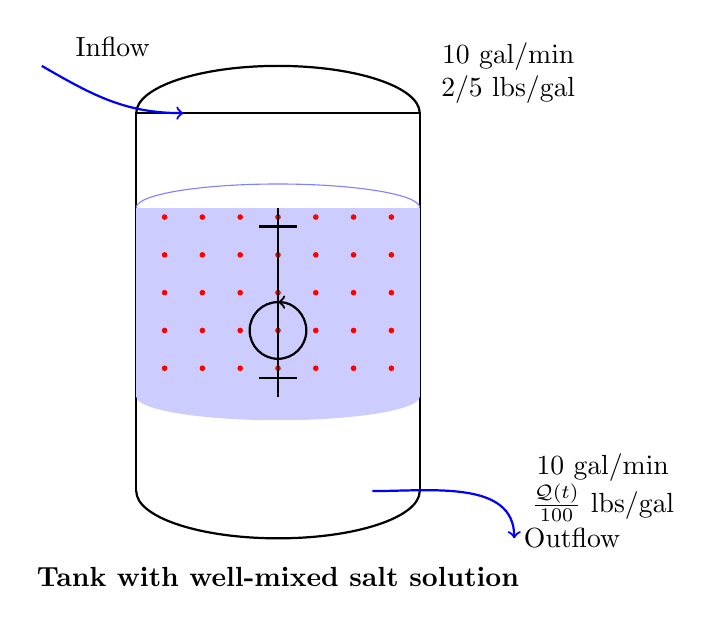
\begin{tikzpicture}[scale=1.2]
        % Tank
        \draw[thick] (0,0) -- (0,4) -- (3,4) -- (3,0);
        \draw[thick] (0,0) arc (180:360:1.5cm and 0.5cm);
        \draw[thick] (0,4) arc (180:0:1.5cm and 0.5cm);
        
        % Water in tank
        \fill[blue!20] (0,1) rectangle (3,3);
        \fill[blue!20] (0,1) arc (180:360:1.5cm and 0.25cm);
        \draw[blue!50] (0,3) arc (180:0:1.5cm and 0.25cm);
        
        % Inflow
        \draw[->, thick, blue] (-1,4.5) to[out=-30,in=180] (0.5,4);
        \node[above] at (-0.25,4.5) {Inflow};
        
        % Outflow
        \draw[->, thick, blue] (2.5,0) to[out=0,in=90] (4,-0.5);
        \node[right] at (4,-0.5) {Outflow};
        
        % Salt particles
        \foreach \x in {0.3,0.7,1.1,1.5,1.9,2.3,2.7}
            \foreach \y in {1.3,1.7,2.1,2.5,2.9}
                \fill[red] (\x,\y) circle (0.03);
        
        % Mixer
        \draw[thick] (1.5,1) -- (1.5,3);
        \draw[thick] (1.3,2.8) -- (1.7,2.8);
        \draw[thick] (1.3,1.2) -- (1.7,1.2);
        \draw[->, thick] (1.5,2) arc (90:450:0.3);
        
        % Labels
        \node[below] at (1.5,-0.7) {\textbf{Tank with well-mixed salt solution}};
        \node[text width=2cm, align=center, above right] at (3,4) {10 gal/min\\2/5 lbs/gal};
        \node[text width=2cm, align=center, below right] at (4,0.5) {10 gal/min\\$\frac{\mathcal{Q}(t)}{100}$ lbs/gal};
    \end{tikzpicture}
    \caption{Diagram of a tank with water inflow, outflow, and well-mixed salt solution}
    \label{fig:tank_mixture}
\end{figure}

\textbf{Example:} Consider a tank with the following properties:

\begin{itemize}
    \item Initial contents: 100 gallons of brine
    \item Initial salt content: 20 lbs dissolved in the brine
    \item Inflow: Brine containing 2/5 lbs/gal of salt at 10 gal/min
    \item Outflow: Well-mixed solution at 10 gal/min
\end{itemize}

\textbf{Problem:} Find a formula for the salt content after $t$ minutes.

\textbf{Solution:} Let $\mathcal{Q}(t)$ be the quantity of salt at time $t$.

\begin{align*}
    \text{Rate of salt inflow} &= 10 \text{ gal/min} \cdot \frac{2}{5} \text{ lbs/gal} = 4 \text{ lbs/min} \\
    \text{Rate of salt outflow} &= 10 \text{ gal/min} \cdot \frac{\mathcal{Q}(t)}{100} \text{ lbs/gal} = \frac{\mathcal{Q}(t)}{10} \text{ lbs/min}
\end{align*}

The rate of change of salt content is the difference between inflow and outflow:

\[
\frac{d\mathcal{Q}}{dt} = \text{salt in} - \text{salt out} = 4 - \frac{\mathcal{Q}(t)}{10}
\]

This is our differential equation. We can solve it using the integrating factor method or separation of variables.

The initial condition is:

\[
\mathcal{Q}(0) = 20 \text{ lbs}
\]

Therefore, our initial value problem (IVP) is:

\[
\begin{cases}
\mathcal{Q}' = 4 - \frac{\mathcal{Q}}{10} \\
\mathcal{Q}(0) = 20
\end{cases}
\]

\textbf{Solve the IVP:} The equation is linear: $\mathcal{Q}' + \frac{1}{10}\mathcal{Q} = 4$

\begin{align*}
    a(t) &= \frac{1}{10} \Rightarrow A(t) = \frac{t}{10} \\[6pt]
    \text{Multiply by } e^{t/10}&: e^{t/10} \mathcal{Q}' + \frac{1}{10}e^{t/10}\mathcal{Q} = 4e^{t/10} \\[6pt]
    \text{Integrate both sides}&: e^{t/10}\mathcal{Q} = 40e^{t/10} + C \\[6pt]
    &\Rightarrow \mathcal{Q} = 40 + Ce^{-t/10}
\end{align*}

Use the initial condition to solve for $C$:
\begin{align*}
    20 &= 40 + C \Rightarrow C = -20
\end{align*}

Therefore, the solution is:
\[
    \mathcal{Q}(t) = 40 - 20e^{-t/10}
\]


\subsection*{Further Questions}

\subsubsection*{Asymptotic Behavior}
As $t \rightarrow \infty$, what happens to $\mathcal{Q}(t)$?

\textbf{Answer:} 
\begin{align*}
    \lim_{t \to \infty} \mathcal{Q}(t) &= \lim_{t \to \infty} (40 - 20e^{-t/10}) \\
    &= 40 - 20 \lim_{t \to \infty} e^{-t/10} \\
    &= 40 - 20(0) = 40 \text{ lbs}
\end{align*}

\subsubsection*{Time to Reach a Specific Amount}
After what time will there be more than 30 lbs of salt in the tank?

\textbf{Answer:} Set $\mathcal{Q}(t) = 30$ lbs and solve for $t$:
\begin{align*}
    30 &= 40 - 20e^{-t/10} \\
    -10 &= -20e^{-t/10} \\
    \frac{1}{2} &= e^{-t/10} \\
    \ln(\frac{1}{2}) &= -\frac{t}{10} \\
    t &= 10\ln(2) \approx 6.93 \text{ minutes}
\end{align*}

\subsection*{General Case}

\begin{figure}[h]
    \centering
    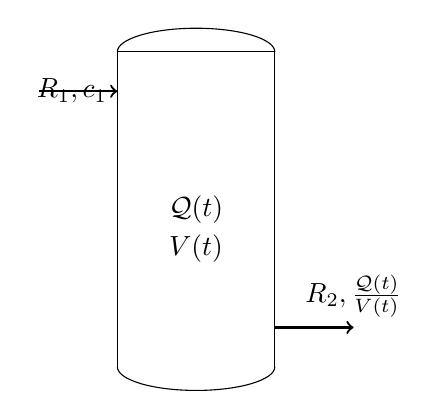
\begin{tikzpicture}
        % Draw cylinder
        \draw (0,0) -- (0,4) -- (2,4) -- (2,0);
        \draw (0,0) arc (180:360:1cm and 0.3cm);
        \draw (0,4) arc (180:0:1cm and 0.3cm);
        
        % Inflow and outflow arrows
        \draw[->,thick] (-1,3.5) -- (0,3.5) node[left] {$R_1, c_1$};
        \draw[->,thick] (2,0.5) -- (3,0.5) node[above] {$R_2, \frac{\mathcal{Q}(t)}{V(t)}$};
        
        % Label contents
        \node at (1,2) {$\mathcal{Q}(t)$};
        \node at (1,1.5) {$V(t)$};
    \end{tikzpicture}
    \caption{Cylinder with inflow and outflow}
\end{figure}

\textbf{Parameters:}
\begin{itemize}
    \item $R_1$: Rate of inflow
    \item $c_1$: Concentration of inflow
    \item $R_2$: Rate of outflow
    \item $\frac{\mathcal{Q}(t)}{V(t)}$: Concentration of outflow
\end{itemize}

\textbf{Initial Conditions:}
\begin{align*}
    \mathcal{Q}(0) &= \mathcal{Q}_0 \\
    V(0) &= V_0
\end{align*}

\textbf{Differential Equations:}
\begin{align*}
    V'(t) &= r_1 - r_2  = v(t) = (r_1 - r_2)t + v_0\\
    \mathcal{Q}'(t) &= r_1c_1 - r_2 \frac{\mathcal{Q}(t)}{V(t)} = r_1c_1 - \frac{r_2q(t)}{(r_1-r_2)t+v0}
\end{align*}

\textbf{Salt Analysis:}
\begin{itemize}
    \item Salt in: $r_1c_1$
    \item Salt out: $\frac{\mathcal{Q}(t)}{V(t)}$
\end{itemize}

\textbf{Population Dynamics:}

Let $P(t)$ be the population at time $t$. Consider the differential equation:
\[
    \frac{dP}{dt} = R(P)P - h(t)
\]
where:
\begin{itemize}
    \item $R(P)$: Growth rate
    \item $h(t)$: Harvest rate
\end{itemize}

\textbf{Exponential Model:}
For the exponential model, we take $h(t) = 0$ and $R(P) = r$ (constant).

The differential equation becomes:
\[
    \frac{dP}{dt} = rP
\]

The general solution is:
\[
    P(t) = Ce^{rt}
\]

With the initial condition $P(0) = P_0$, we get:
\[
    P(t) = P_0e^{rt}
\]

\textbf{Example 1: Monkey Population Growth}

Consider a population of monkeys with the following characteristics:
\begin{itemize}
    \item Initial population: 100 monkeys
    \item Growth rate: 4\% per year
    \item Immigration: 8 new monkeys join from surrounding tribes every year
\end{itemize}

The Initial Value Problem (IVP) describing this system is:

\begin{align*}
    \frac{dM}{dt} &= 0.04M + 8 \\
    M(0) &= 100
\end{align*}

where $M(t)$ represents the number of monkeys at time $t$.

\textbf{Solution:} $M(t) = 300e^{0.04t} - 200$

\vspace{0.5cm}

\textbf{Example 2: Rabbit Population Growth}

A population of rabbits doubles in size every year.

\textbf{Question:} What is the growth rate assuming exponential growth?

\textbf{Solution:}
Let's assume the population follows the exponential growth model:

\[P(t) = P_0e^{rt}\]

where:
\begin{itemize}
    \item $P(t)$ is the population at time $t$
    \item $P_0$ is the initial population
    \item $r$ is the growth rate
    \item $t$ is time in years
\end{itemize}

Given:
\begin{align*}
    P(0) &= P_0 \\
    P(1) &= 2P_0
\end{align*}

Substituting into our model:

\[2P_0 = P_0e^r\]

Simplifying:

\[2 = e^r\]

Taking the natural logarithm of both sides:

\[r = \ln(2) \approx 0.693\]

Therefore, the growth rate is approximately 69.3\% per year.

\textbf{Logistic Model:} This model accounts for finite resources and competition.

\begin{equation}
    \frac{dp}{dt} = (r-ap)p
\end{equation}

where:
\begin{itemize}
    \item $R(p) = r-ap$ is the per capita growth rate
    \item When $p$ is small, $R(p) \approx r$
    \item As $p$ grows, $R(p)$ decreases
    \item At $p = \frac{r}{a}$, $R(p) = 0$ (this is called the carrying capacity)
\end{itemize}

\textbf{Stationary solutions:} Set $(r-ap) = 0$
\[\Rightarrow p = 0 \text{ or } p = \frac{r}{a}\]

\textbf{Phase-line portrait:}

\begin{figure}[h]
    \centering
    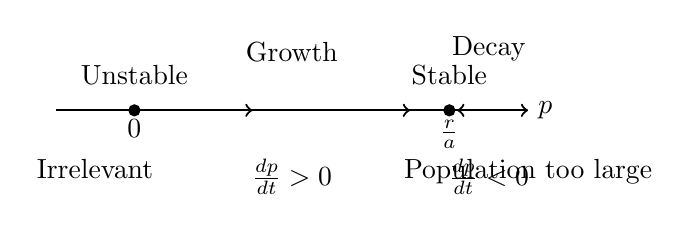
\begin{tikzpicture}
        % Main axis
        \draw[->, thick] (-1,0) -- (5,0) node[right] {$p$};
        
        % Equilibrium points
        \draw[fill] (0,0) circle (2pt) node[below] {0};
        \draw[fill] (4,0) circle (2pt) node[below] {$\frac{r}{a}$};
        
        % Arrows on the line
        \draw[->, thick] (0.5,0) -- (1.5,0);
        \draw[->, thick] (2.5,0) -- (3.5,0);
        \draw[->, thick] (4.5,0) -- (4.1,0);
        
        % Labels for equilibrium points
        \node[above] at (0,0.2) {Unstable};
        \node[above] at (4,0.2) {Stable};
        
        % Labels for regions
        \node[above] at (2,0.5) {Growth};
        \node[below] at (2,-0.5) {$\frac{dp}{dt} > 0$};
        
        \node[above] at (4.5,0.5) {Decay};
        \node[below] at (4.5,-0.5) {$\frac{dp}{dt} < 0$};
        
        % Additional labels
        \node[below] at (-0.5,-0.5) {Irrelevant};
        \node[below] at (5,-0.5) {Population too large};
    \end{tikzpicture}
    \caption{Phase-line portrait for the logistic model}
\end{figure}


\subsection*{Additional Phase Line Portraits}

Here are three more examples of phase line portraits:

\begin{enumerate}
    \item Simple linear model:
    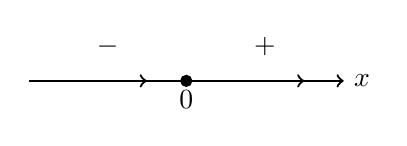
\begin{tikzpicture}[baseline]
        \draw[->, thick] (-2,0) -- (2,0) node[right] {$x$};
        \draw[fill] (0,0) circle (2pt) node[below] {0};
        \draw[->, thick] (-1.5,0) -- (-0.5,0);
        \draw[->, thick] (0.5,0) -- (1.5,0);
        \node[above] at (-1,0.2) {$-$};
        \node[above] at (1,0.2) {$+$};
    \end{tikzpicture}

    \item Logistic model:
    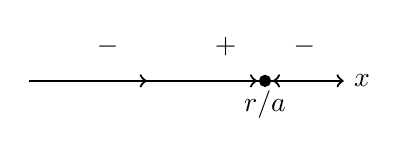
\begin{tikzpicture}[baseline]
        \draw[->, thick] (-2,0) -- (2,0) node[right] {$x$};
        \draw[fill] (1,0) circle (2pt) node[below] {$r/a$};
        \draw[->, thick] (-1.5,0) -- (-0.5,0);
        \draw[->, thick] (0.5,0) -- (0.9,0);
        \draw[->, thick] (1.5,0) -- (1.1,0);
        \node[above] at (-1,0.2) {$-$};
        \node[above] at (0.5,0.2) {$+$};
        \node[above] at (1.5,0.2) {$-$};
    \end{tikzpicture}


    \item Reversed logistic model:
    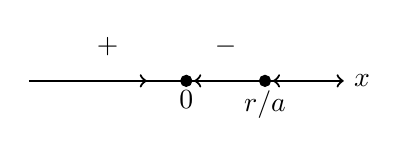
\begin{tikzpicture}[baseline]
        \draw[->, thick] (-2,0) -- (2,0) node[right] {$x$};
        \draw[fill] (0,0) circle (2pt) node[below] {0};
        \draw[fill] (1,0) circle (2pt) node[below] {$r/a$};
        \draw[->, thick] (-1.5,0) -- (-0.5,0);
        \draw[->, thick] (0.5,0) -- (0.1,0);
        \draw[->, thick] (1.5,0) -- (1.1,0);
        \node[above] at (-1,0.2) {$+$};
        \node[above] at (0.5,0.2) {$-$};
    \end{tikzpicture}

\end{enumerate}


Variant logistic model:

$\frac{dp}{dt} = -(r-ap)p$

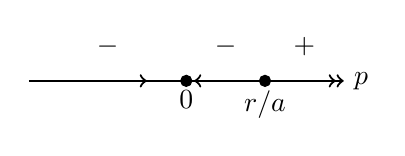
\begin{tikzpicture}[baseline]
    \draw[->, thick] (-2,0) -- (2,0) node[right] {$p$};
    \draw[fill] (0,0) circle (2pt) node[below] {0};
    \draw[fill] (1,0) circle (2pt) node[below] {$r/a$};
    \draw[->, thick] (-1.5,0) -- (-0.5,0);
    \draw[->, thick] (0.5,0) -- (0.1,0);
    \draw[->, thick] (1.5,0) -- (1.9,0);
    \node[above] at (-1,0.2) {$-$};
    \node[above] at (0.5,0.2) {$-$};
    \node[above] at (1.5,0.2) {$+$};
\end{tikzpicture}

\noindent This phase line portrait for $\frac{dp}{dt} = -(r-ap)p$ shows:
\begin{itemize}
    \item Two equilibrium points: at $p=0$ and $p=r/a$
    \item For $p < 0$, $\frac{dp}{dt} < 0$, so $p$ decreases (moves left)
    \item For $0 < p < r/a$, $\frac{dp}{dt} < 0$, so $p$ decreases (moves left)
    \item For $p > r/a$, $\frac{dp}{dt} > 0$, so $p$ increases (moves right)
\end{itemize}

This describes a context where a population needs a certtin critical size r/a to be able to grow otherwise it will die out.



\section*{Lecture 5, Tuesday 9/10/2024}

\subsection*{I.6 Motion: Falling Objects (continued)}

Consider an object with mass $m$ and force $F$ acting on it. Newton's Second Law of Motion states:

\[F = ma\]

where $a$ is the acceleration, defined as:

\[a = \frac{dv(t)}{dt}\]

and $v(t)$ is the velocity.

For our analysis, we will use the following coordinate system:

\begin{tikzpicture}
    \draw[->] (0,-2) -- (0,2) node[above] {$y$};
    \draw[->] (0,1.5) -- (0,2) node[right] {$+$};
    \draw[->] (0,-1.5) -- (0,-2) node[right] {$-$};
\end{tikzpicture}


For falling objects, the total force is composed of gravity and drag:

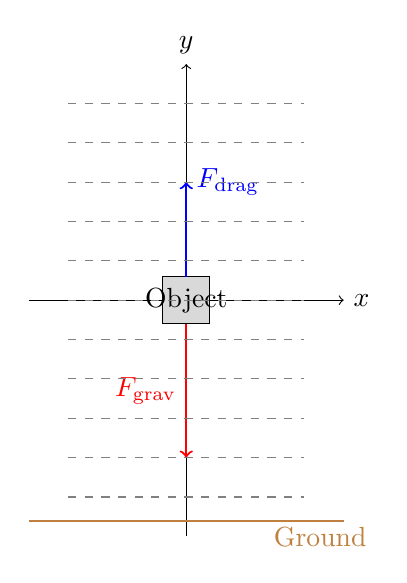
\begin{tikzpicture}
    % Coordinate system
    \draw[->] (0,-3) -- (0,3) node[above] {$y$};
    \draw[->] (-2,0) -- (2,0) node[right] {$x$};
    
    % Object (more realistic shape)
    \draw[fill=gray!30] (-0.3,-0.3) rectangle (0.3,0.3);
    \node at (0,0) {Object};
    
    % Gravity force (longer arrow)
    \draw[->, thick, red] (0,-0.3) -- (0,-2) node[left, midway] {$F_\text{grav}$};
    
    % Drag force (straight arrow to show air resistance)
    \draw[->, thick, blue] 
        (0,0.3) -- (0,1.5) node[right] {$F_\text{drag}$};
    
    % Air flow lines to indicate drag
    \foreach \y in {-2.5,-2,...,2.5}
    {
        \draw[gray, dashed] (-1.5,\y) -- (1.5,\y);
    }
    
    % Ground reference
    \draw[thick, brown] (-2,-2.8) -- (2,-2.8);
    \node[brown] at (1.7,-3) {Ground};
\end{tikzpicture}

Where:
\begin{align*}
    F_\text{grav} &= \text{force from gravity} = mg \\
    F_\text{drag} &= \text{drag force} = -cv^2
\end{align*}

Here, $g = -9.8 \text{ m/s}^2$, $c$ is a constant, and $v$ is velocity.

Therefore, our ODE model for a falling object is:

\[ma = m\frac{dv}{dt} = mg - cv^2\]


\noindent
Let $c$ be the drag constant.

\vspace{0.5em}

Cancelling out $m$, we get:
\[
v' = g + cv^2
\]

This is a non-linear equation, but it is separable.

\vspace{0.5em}

Stationary solutions are found by solving:
\[
g + cv^2 = 0 \quad \Rightarrow \quad v = \pm\sqrt{-g/c}
\]

For falling objects, we are interested in the negative velocity solution. Thus,
\[
v_\infty = -\sqrt{-g/c}
\]
is called the terminal velocity.

\vspace{0.5em}

\begin{center}
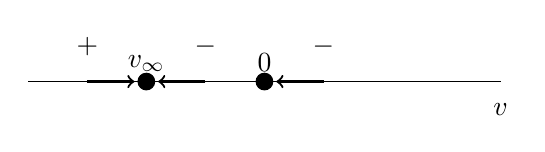
\begin{tikzpicture}[scale=1.5]
    % Draw the horizontal line
    \draw[-] (-2,0) -- (2,0);
    
    % Add labels and points
    \node[below] at (2,-0.1) {$v$};
    \filldraw (0,0) circle (2pt) node[above] {$0$};
    \filldraw (-1,0) circle (2pt) node[above] {$v_\infty$};
    
    % Add arrows to show direction
    \draw[->, thick] (-0.5,0) -- (-0.9,0);
    \draw[->, thick] (0.5,0) -- (0.1,0);
    \draw[->, thick] (-1.5,0) -- (-1.1,0);
    
    % Add signs
    \node at (0.5,0.3) {$-$};
    \node at (-0.5,0.3) {$-$};
    \node at (-1.5,0.3) {$+$};
\end{tikzpicture}
\end{center}

This horizontal phase line portrait shows:
\begin{itemize}
    \item The equilibrium points at $v=0$ and $v=v_\infty$
    \item Arrows indicating the direction of change
    \item Signs showing whether $v'$ is positive or negative in each region
\end{itemize}

We can observe that:
\begin{itemize}
    \item For $v > 0$, $v'$ is negative, so $v$ decreases towards 0
    \item For $v_\infty < v < 0$, $v'$ is still negative, so $v$ continues to decrease towards $v_\infty$
    \item For $v < v_\infty$, $v'$ becomes positive, so $v$ increases back towards $v_\infty$
\end{itemize}

This confirms that $v_\infty$ is indeed the terminal velocity, as the system will eventually settle at this value regardless of the initial conditions.


A skydiver with mass $m = 60\text{ kg}$ jumps from an airplane and assumes a position with drag coefficient $c = 0.002\text{ m}^{-1}$. Find her terminal velocity.

\textbf{Solution:}

$v(0) = 0, c = 0.002, g = -9.8$

$\Rightarrow v' = g+0.002v^2$

terminal velocity $v_\infty = -\sqrt{\frac{-g}{c}}$

To find the terminal velocity, we use the formula derived earlier:

\[
v_\infty = -\sqrt{\frac{-g}{c}}
\]


Substituting the given values:

\[
v_\infty = -\sqrt{\frac{9.8\text{ m/s}^2}{0.002\text{ m}^{-1}}} = -70.0\text{ m/s}
\]

Therefore, the skydiver's terminal velocity is approximately 70.0 m/s (or 252 km/h) downward.

Now, let's solve the ODE analytically:

Rewrite the ODE:
\begin{align*}
v' &= g + cv^2 \\
   &= c\left(\frac{g}{c} + v^2\right) \\
   &= c(v^2 - v_\infty^2) \\
   &= c(v - v_\infty)(v + v_\infty)
\end{align*}

Separate variables:
\[
\frac{v'}{(v - v_\infty)(v + v_\infty)} = c
\]

Integrate both sides:
\[
\int \frac{v'}{(v - v_\infty)(v + v_\infty)} \, dv = \int c \, dt
\]

Using partial fractions decomposition:
\[
\frac{1}{2v_\infty}\left(\ln|v - v_\infty| - \ln|v + v_\infty|\right) = ct + C_0
\]

Apply initial condition $v(0) = 0$:
\[
C_0 = \frac{1}{2v_\infty}\left(\ln|-v_\infty| - \ln|v_\infty|\right) = 0
\]

Therefore, the solution is:
\[
\ln\left|\frac{v - v_\infty}{v + v_\infty}\right| = 2cv_\infty t
\]


\subsection{I.7: Numerical Methods}

Consider the initial value problem:
\[
y' = f(t, y), \quad y(t_I) = y_I
\]

Our goal is to approximate $y(t_f)$, where $t_f > t_I$.

To do this, we divide the interval $[t_I, t_f]$ into $n$ equal steps:

\begin{center}
\begin{tikzpicture}
\draw[->] (0,0) -- (10,0) node[right] {$t$};
\draw (0,-0.2) -- (0,0.2) node[above] {$t_I = t_0$};
\draw (2,-0.2) -- (2,0.2) node[above] {$t_1$};
\draw (4,-0.2) -- (4,0.2) node[above] {$t_2$};
\draw (8,-0.2) -- (8,0.2) node[above] {$t_{N-1}$};
\draw (10,-0.2) -- (10,0.2) node[above] {$t_N = t_f$};
\draw[dotted] (5,0) -- (7,0);
\end{tikzpicture}
\end{center}

We then use an iterative process to approximate the solution:

\begin{enumerate}
    \item Use $y(t_0) = y_I$ to approximate $y(t_1)$
    \item Use the approximation of $y(t_1)$ to approximate $y(t_2)$
    \item $\vdots$
    \item Use the approximation of $y(t_{N-1})$ to approximate $y(t_N)$
\end{enumerate}

This process forms the basis of numerical methods for solving differential equations.


For good methods, the accuracy of the approximation increases as N increases.

We will use uniform step sizes:

\[
\text{step size} = h = \frac{t_f - t_I}{N}
\]

\[
t_i = t_I + ih \quad \text{for } i = 0, 1, 2, \ldots, N
\]

\textbf{Euler method:}

Idea: The derivative can be approximated by the difference quotient
\[
f'(t) \approx \lim_{h \to 0} \frac{f(t+h) - f(t)}{h}
\]

For small $h$, we have the approximation:
\[
f(t+h) \approx f(t) + hf'(t)
\]

% (A graph would be inserted here)

If $y(t)$ is the solution to $y' = f(t,y)$ with $y(t_i) = y_i$, then:

\[
y(t_i + h) \approx y(t_i) + hy'(t_i) = y(t_i) + hf(t_i, y(t_i))
\]

Thus,
\[
y(t_1) \approx y(t_0) + hf(t_0, y(t_0))
\]
\[
y(t_2) \approx y(t_1) + hf(t_1, y(t_1))
\]

\textbf{Algorithm:}
\begin{enumerate}
    \item Set $y_0 = y_I$
    \item For $i = 1, 2, \ldots, N$:
    \[
    y_i = y_{i-1} + hf(t_{i-1}, y_{i-1})
    \]
    \item Then $y(t_f) \approx y(t_N) = y_N$
\end{enumerate}


\textbf{Example:} Let $y(t)$ be the solution to $y' = t^2 + y^2$, $y(0) = 1$.

Approximate $y(0.2)$ with step size $h = 0.1$ using the Euler method.

\textbf{Solution:}
\begin{align*}
    t_0 &= 0, \quad t_1 = 0.1, \quad t_2 = 0.2 \\[6pt]
    y_0 &= 1 \\[6pt]
    y_1 &= y_0 + hf(t_0, y_0) = 1 + 0.1(0^2 + 1^2) = 1.1 \\[6pt]
    y_2 &= y_1 + hf(t_1, y_1) = 1.1 + 0.1((0.1)^2 + 1.1^2) = 1.222
\end{align*}

Therefore, $y(0.2) \approx 1.222$.


\textbf{Note:} In textbooks, this is often referred to as the explicit Euler method. We will not cover the implicit Euler method in this course.

The Euler Method approximation is derived from a Taylor series expansion:

\[
y(t+h) = y(t) + hy'(t) + \frac{h^2}{2}y''(t) + \cdots
\]

The terms $\frac{h^2}{2}y''(t) + \cdots$ are of order $O(h^2)$, which means they approach zero faster than $h$ as $h \to 0$.



\textbf{Error Analysis:}
\begin{itemize}
    \item $O(h^2)$ represents the local error, i.e., the error at each step.
    \item The global error (total error) is the sum of the local errors: $N \cdot O(h^2)$.
    \item Since $N = \frac{T_f - T_I}{h} = \frac{\text{constant}}{h}$, we have:
    \[
    \frac{\text{constant}}{h} \cdot O(h^2) = O(h)
    \]
\end{itemize}

\textbf{Upshot:} ``Error is $O(h)$" implies that if we scale $h$ by a constant $c$, the error should also scale by $c$.

\subsection*{Higher-order Taylor Series Approximations}

\textbf{Example: Order 2}

The second-order Taylor series approximation for $y(t+h)$ is:

\[
y(t+h) = y(t) + hy'(t) + \frac{h^2}{2} y''(t) + O(h^3)
\]

If $y(t)$ is the solution to $y' = f(t,y)$, then:

\begin{align*}
y'(t) &= f(t,y) \\
y''(t) &= \frac{d}{dt}f(t,y(t)) = \frac{\partial f}{\partial t}(t,y(t)) + \frac{\partial f}{\partial y}(t,y(t)) \cdot y'(t)
\end{align*}

Substituting these into the Taylor series approximation:

\[
y(t+h) \approx y(t) + hf(t,y(t)) + \frac{h^2}{2} \left(\frac{\partial f}{\partial t}(t,y(t)) + \frac{\partial f}{\partial y}(t,y(t)) \cdot f(t,y(t))\right)
\]

This method would have error $O(h^2)$


\section*{Lecture 6, Thursday 9/12/2024}


\subsection*{I.7 (continued): Integral Approximations}

\textbf{Recall:} For a function $f(t)$, we have:
\[
f(t+h) - f(t) = \int_t^{t+h} f'(x) \, dx
\]

Therefore,
\[
f(t+h) = f(t) + \int_t^{t+h} f'(x) \, dx
\]

We can approximate this integral in two ways:

\subsubsection*{1. Left Sum (Euler Method)}

\begin{figure}[h]
    \centering
    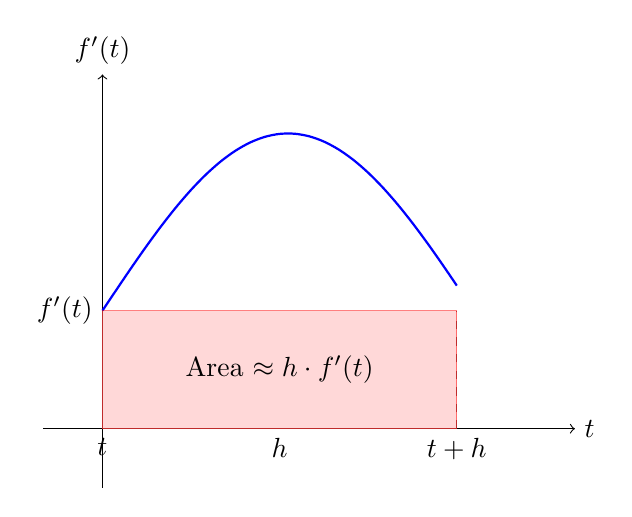
\begin{tikzpicture}[scale=1.5]
        \draw[->] (-0.5,0) -- (4,0) node[right] {$t$};
        \draw[->] (0,-0.5) -- (0,3) node[above] {$f'(t)$};
        \draw[domain=0:3, smooth, variable=\x, blue, thick] plot ({\x}, {1+1.5*sin(\x r)});
        \draw[dashed] (0,0) -- (0,1);
        \draw[dashed] (3,0) -- (3,1);
        \filldraw[fill=red!30, draw=red, opacity=0.5] (0,0) rectangle (3,1);
        \node at (1.5,0.5) {Area $\approx h \cdot f'(t)$};
        \node[below] at (1.5,0) {$h$};
        \node[left] at (0,1) {$f'(t)$};
        \node[below] at (0,0) {$t$};
        \node[below] at (3,0) {$t+h$};
    \end{tikzpicture}
    \caption{Left sum approximation}
\end{figure}

Approximating the integral using a rectangle:
\begin{itemize}
    \item Area of rectangle: $h \cdot f'(t)$
    \item Approximation: $f(t+h) \approx f(t) + h f'(t)$
\end{itemize}

This approximation forms the basis of the Euler method.

\subsubsection*{2. Trapezoid Method}

\begin{figure}[h]
    \centering
    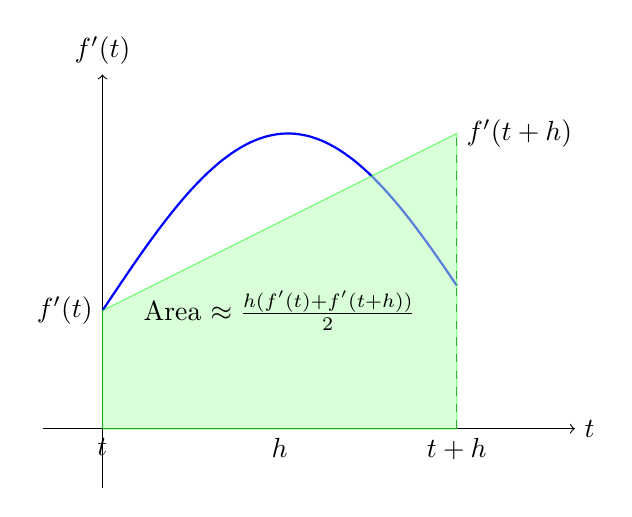
\begin{tikzpicture}[scale=1.5]
        \draw[->] (-0.5,0) -- (4,0) node[right] {$t$};
        \draw[->] (0,-0.5) -- (0,3) node[above] {$f'(t)$};
        \draw[domain=0:3, smooth, variable=\x, blue, thick] plot ({\x}, {1+1.5*sin(\x r)});
        \draw[dashed] (0,0) -- (0,1);
        \draw[dashed] (3,0) -- (3,2.5);
        \filldraw[fill=green!30, draw=green, opacity=0.5] (0,0) -- (0,1) -- (3,2.5) -- (3,0) -- cycle;
        \node at (1.5,1) {Area $\approx \frac{h(f'(t) + f'(t+h))}{2}$};
        \node[below] at (1.5,0) {$h$};
        \node[left] at (0,1) {$f'(t)$};
        \node[right] at (3,2.5) {$f'(t+h)$};
        \node[below] at (0,0) {$t$};
        \node[below] at (3,0) {$t+h$};
    \end{tikzpicture}
    \caption{Trapezoid approximation}
\end{figure}

For a trapezoid with bases $h_1$ and $h_2$ and width $w$:
\[
\text{Area} = \frac{w(h_1 + h_2)}{2}
\]

Applying this to our integral:
\[
\int_t^{t+h} f'(x) \, dx \approx \frac{h(f'(t) + f'(t+h))}{2}
\]

Therefore,
\[
f(t+h) \approx f(t) + \frac{h(f'(t) + f'(t+h))}{2}
\]

\[
f(t+h) \approx f(t) + h(f'(t) + f'(t+h))/2
\]

Now, let $Y(t)$ be the solution to the differential equation:
\[
y' = f(t,y), \quad y(t_I) = y_i
\]
We want to find $Y(t_F)$. Choose $N$ steps, with step size $h = \frac{t_F - t_I}{N}$.

Define $t_k = t_I + kh$ for $k = 0, 1, \ldots, N$.

Initialize $y_0 = y_i$.

The trapezoid method suggests:
\[
y_{k+1} = y_k + \frac{h}{2}[f(t_k, y_k) + f(t_{k+1}, y_{k+1})]
\]

However, we can't use $y_{k+1}$ to compute $y_{k+1}$. Instead, we replace $y_{k+1}$ in $f(t_{k+1}, y_{k+1})$ with an Euler step approximation:

\[
y_{k+1} \approx y_k + hf(t_k, y_k)
\]

Therefore, we set:
\[
y_{k+1} = y_k + \frac{h}{2}[f(t_k, y_k) + f(t_{k+1}, y_k + hf(t_k, y_k))]
\]

It turns out that the global error of this method is $O(h^2)$.

This is called range-trapezoid method.


\subsection*{Example: Trapezoid Method}

Consider the differential equation:
\[
y' = t^2 + y^2, \quad y(0) = 1
\]

Let's estimate $y(0.2)$ using the trapezoid method with $h = 0.1$.

\textbf{Solution:} 
We have $f(t, y) = t^2 + y^2$, $h = 0.1$, $t_0 = 0$, $t_1 = 0.1$, and $t_2 = 0.2$.

\begin{align*}
y_1 &= y_0 + \frac{h}{2}[f(t_0, y_0) + f(t_1, y_0 + hf(t_0, y_0))] \\
&= 1 + \frac{0.1}{2}[(0^2 + 1^2) + (0.1^2 + (1 + 0.1 \cdot 1^2)^2)] \\
&= 1 + 0.1 \cdot \frac{1 + 0.01 + 1.21}{2} \\
&= 1 + 0.1 \cdot 1.11 \\
&= 1.111
\end{align*}

\begin{align*}
y_2 &= y_1 + \frac{h}{2}[f(t_1, y_1) + f(t_2, y_1 + hf(t_1, y_1))] \\
&= 1.111 + \frac{0.1}{2}[(0.1^2 + 1.111^2) + (0.2^2 + (1.111 + 0.1 \cdot 1.111^2)^2)] \\
&= 1.111 + 0.1 \cdot \frac{0.010201 + 1.234543}{2} \\
&= 1.111 + 0.1 \cdot 1.122372 \\
&\approx 1.248
\end{align*}

\subsection*{Range-Midpoint Method}

For the range-midpoint method, we use the formula:
\[
y_{k+1} = y_k + hf\left(t_k + \frac{h}{2}, y_k + \frac{h}{2}f(t_k, y_k)\right)
\]

The global error for this method is $O(h^2)$.

\textit{Note: See textbook page 13 for an example.}

\subsection*{Exact ODEs \& Integrating Factors}

Consider a first-order ODE of the form $\frac{dy}{dx} = f(x,y)$.

\textbf{Question:} When do we have an implicit solution $H(x,y) = c$?

Differentiating both sides with respect to $x$, remembering that $y = y(x)$:
\[
\frac{\partial H}{\partial x} + \frac{\partial H}{\partial y} \cdot \frac{dy}{dx} = 0
\]

This leads to the general form of an exact ODE:
\[
M(x,y) + N(x,y)\frac{dy}{dx} = 0
\]

Alternatively written as:
\[
M(x,y)dx + N(x,y)dy = 0
\]

\textbf{Question:} When can we find a function $H(x,y)$ with $\frac{\partial H}{\partial x} = M$ and $\frac{\partial H}{\partial y} = N$?

If $H$ has continuous second derivatives, then:
\[
\frac{\partial^2 H}{\partial x \partial y} = \frac{\partial^2 H}{\partial y \partial x}
\]

\textbf{Answer:} If the domain of $M$ and $N$ has no "holes" and $\frac{\partial M}{\partial y} = \frac{\partial N}{\partial x}$, then we can find a function $H(x,y)$ such that $\frac{\partial H}{\partial x} = M$ and $\frac{\partial H}{\partial y} = N$.

Such an ODE is called exact.

\subsection*{Example 1: Solve the IVP $(e^x y + 2x) + (2y + e^x)y' = 0$, $y(0) = 0$}

\textbf{Solution:} We have $M = e^x y + 2x$, $N = 2y + e^x$. Let's check if the ODE is exact:

\begin{align*}
    \frac{\partial M}{\partial y} &= e^x \\
    \frac{\partial N}{\partial x} &= e^x
\end{align*}

These are equal, so the ODE is exact.

We want to find $H(x,y)$ such that $\frac{\partial H}{\partial x} = M$ and $\frac{\partial H}{\partial y} = N$.

From $\frac{\partial H}{\partial x} = M$:
\[
    H(x,y) = \int (e^x y + 2x) \, dx = e^x y + x^2 + C(y)
\]

From $\frac{\partial H}{\partial y} = N$:
\[
    e^x + C'(y) = 2y + e^x
\]

Solving for $C(y)$:
\[
    C'(y) = 2y \implies C(y) = y^2
\]

Therefore, $H(x,y) = e^x y + x^2 + y^2 = C$ is our general solution to the ODE.

Applying the initial condition $y(0) = 0$:
\[
    e^0 \cdot 0 + 0^2 + 0^2 = C \implies C = 0
\]

So the solution to the IVP is $e^x y + x^2 + y^2 = 0$.

\textbf{Alternative approach:} Start with $\frac{\partial H}{\partial y} = 2y + e^x$
\[
    H(x,y) = y^2 + e^x y + C(x)
\]
Then plug $\frac{\partial H}{\partial x} = e^x y + C'(x)$ into $M$ and solve for $C(x)$.

\subsection*{Example 2: Solve $(3t^2 y + 8ty^2) dt + (t^3 + 8t^2 y + 12t^2 y^2) dy = 0$}

\textbf{Solution:} We have $M = 3t^2 y + 8ty^2$, $N = t^3 + 8t^2 y + 12t^2 y^2$

Let's check if the ODE is exact:
\begin{align*}
    \frac{\partial M}{\partial y} &= 3t^2 + 16ty \\
    \frac{\partial N}{\partial t} &= 3t^2 + 16ty
\end{align*}

These are equal, so the ODE is exact.

We're looking for $H(t,y)$ such that $\frac{\partial H}{\partial t} = M$ and $\frac{\partial H}{\partial y} = N$.

From $\frac{\partial H}{\partial y} = N$:
\[
    H(t,y) = t^3 y + 4t^2 y^2 + C(t)
\]

Now, let's use $\frac{\partial H}{\partial t} = M$:
\begin{align*}
    \frac{\partial H}{\partial t} &= 3t^2y + 8t y^2 + C'(t) \\
    3t^2y + 8t y^2 + C'(t) &= 3t^2 y + 8ty^2
\end{align*}

Comparing the two sides, we see that $C'(t) = 0$, which means $C(t) = K$, where $K$ is a constant.

Therefore, the general solution is:
\[
    H(t,y) = t^3 y + 4t^2 y^2+4y^3 = C
\]

This is the implicit form of the general solution to the given ODE.

\section*{Lecture 7, Tuesday 9/17/2024}


\subsection*{Quiz 3 - I.6.3, I.7, I.9(.1-.2)}

\subsubsection*{I.9 continued}

\textbf{Example:} \(\frac{dy}{dt} = -\frac{y \sin(ty)}{t \sin(ty) + y}\)

\textbf{Solution:} 
\[
(t \sin(ty) + y) \frac{dy}{dt} = -y \sin(ty) \implies y \sin(ty) + (t \sin(ty) + y) \frac{dy}{dt} = 0
\]

Let \( M = y \sin(ty) \) and \( N = t \sin(ty) + y \).

\[
\frac{\partial M}{\partial y} = \sin(ty) + ty \cos(ty)
\]
\[
\frac{\partial N}{\partial t} = \sin(ty) + ty \cos(ty)
\]

Since \(\frac{\partial M}{\partial y} = \frac{\partial N}{\partial t}\), the ODE is exact.

We seek \( H(t, y) \) such that \(\frac{\partial H}{\partial t} = M\) and \(\frac{\partial H}{\partial y} = N\).

From \(\frac{\partial H}{\partial y} = N\):
\[
H(t, y) = \int y \sin(ty) \, dy = -\cos(ty) + C(y)
\]

Now, using \(\frac{\partial H}{\partial t} = M\):
\[
\frac{\partial H}{\partial t} = t \sin(ty) \cos(ty) + C'(y) = t \sin(ty) + y
\]

Thus, 
\[
C'(y) = y \implies C(y) = \frac{y^2}{2} + K
\]

Thus, the general solution is:
\[
H(t, y) = -\cos(ty) + \frac{y^2}{2} = C
\]


\subsection*{Integrating Factors}

\textbf{Example:} \(2ty + (2t^2 - e^y)y' = 0\)

Find the general solution.

Let \( M = 2t \) and \( N = 2t^2 - e^y \).

Check:
\[
\frac{\partial M}{\partial y} = 0, \quad \frac{\partial N}{\partial t} = 4t
\]

Since \(\frac{\partial M}{\partial y} \neq \frac{\partial N}{\partial t}\), the ODE is not exact.

Try multiplying the entire equation by \( y \):
\[
2ty^2 + (2yt^2 - ye^y)y' = 0
\]

Now, let \( M = 2ty \) and \( N = 2yt^2 - ye^y \).

Check again:
\[
\frac{\partial M}{\partial y} = 2t, \quad \frac{\partial N}{\partial t} = 4ty
\]

Now the ODE is exact.

Solve:
\[
t^2y^2 - (y - 1)e^y = C
\]

This \( y \) is called an integrating factor.

Compare with the standard form:
\[
y' + a(t)y = 0
\]

Multiplying by an integrating factor \( \rho \):
\[
\rho y' + \rho a(t)y = 0
\]

Let \( \rho = e^{A(t)} \), then:
\[
e^{A(t)}y' + a(t)e^{A(t)}y = 0
\]

In general, for \( M + N \frac{dy}{dx} = 0 \) which is not exact, we want to multiply by a function \( \rho(x, y) \) so that \( \rho M + \rho N \frac{dy}{dx} = 0 \) is exact.

The function \( \rho \) is called an integrating factor.

The equation is exact if:
\[
\frac{\partial (\rho M)}{\partial y} = \frac{\partial (\rho N)}{\partial x}
\]

This leads to the partial differential equation (PDE):
\[
\rho_y M + \rho \frac{\partial M}{\partial y} = \rho_x N + \rho \frac{\partial N}{\partial x}
\]

Solving this PDE can be very challenging.

In order to solve, we make an assumption:

either (1) \(\rho\) is only a function of \(x\)

\[
\rho_x = \rho', \quad \rho_y = 0
\]

or (2) \(\rho\) is only a function of \(y\)

\[
\rho_x = 0, \quad \rho_y = \rho'
\]

For example, consider the equation:
\[
2xy + (2x^2 - e^y) \frac{dy}{dx} = 0
\]

Here, \(M = 2x\) and \(N = 2x^2 - e^y\).

We look for an integrating factor \(\rho\) such that:
\[
\frac{\partial}{\partial y} (\rho M) = \frac{\partial}{\partial x} (\rho N)
\]

This gives:
\[
\rho_y M + \rho \frac{\partial M}{\partial y} = \rho_x N + \rho \frac{\partial N}{\partial x}
\]

Substituting \(M\) and \(N\):
\[
\rho_y (2xy) + \rho (2x) = \rho_x (2x^2 - e^y) + \rho (4x)
\]

Assuming \(\rho\) is only a function of \(y\):
\[
\rho_x = 0, \quad \rho_y = \rho'
\]

This simplifies to:
\[
\rho' (2xy) + \rho (2x) = \rho (4x)
\]

Which reduces to:
\[
2xy \rho' = 2x \rho
\]

Solving for \(\rho\):
\[
\rho' = \frac{\rho}{y}
\]

Integrating both sides:
\[
\int \frac{1}{\rho} d\rho = \int \frac{1}{y} dy
\]

This gives:
\[
\ln|\rho| = \ln|y| + C
\]

Thus:
\[
|\rho| = c|y|
\]

We can choose \(\rho = y\).



\textbf{Example:} Find an integrating factor for \((1 + 3x^2 \sin y) - (x \cot y) y' = 0\)

We have:
\[
M = 1 + 3x^2 \sin y, \quad N = -x \cot y
\]

Calculating the partial derivatives:
\[
M_y = 3x^2 \cos y, \quad N_x = -\cot y
\]

Since \(M_y \neq N_x\), we look for an integrating factor \(\rho\).

We start with:
\[
(\rho M)_y = (\rho N)_x
\]

Expanding this, we get:
\[
\rho_y M + \rho M_y = \rho_x N + \rho N_x
\]

Substituting \(M\) and \(N\):
\[
\rho_y (1 + 3x^2 \sin y) + \rho (3x^2 \cos y) = \rho_x (-x \cot y) + \rho (-\cot y)
\]

First, try \(\rho = \rho(x)\):
\[
\rho_y = 0, \quad \rho_x = \rho' = \frac{d\rho}{dx}
\]

This simplifies to:
\[
\rho (3x^2 \cos y) = \rho' x \cot y + \rho \cot y
\]

Multiplying by \(\tan y\):
\[
\rho (3x^2 \sin y) = x \rho' + \rho
\]

Rearranging:
\[
x \rho' = \rho (3x^2 \sin y - 1)
\]

This gives:
\[
\rho' = \frac{\rho (3x^2 \sin y - 1)}{x}
\]

Since the expression for \(\frac{d\rho}{dx}\) has both \(x\) and \(y\), our assumption must not work.

Next, try \(\rho = \rho(y)\):
\[
\rho_x = 0, \quad \rho_y = \rho' = \frac{d\rho}{dy}
\]

This simplifies to:
\[
\rho' (1 + 3x^2 \sin y) + \rho (3x^2 \cos y) = \rho (-x \cot y)
\]

Rearranging:
\[
\rho' (1 + 3x^2 \sin y) = \rho (-\cot y - 3x^2 \cos y)
\]

This gives:
\[
\rho' = \frac{-\rho (\cot y + 3x^2 \cos y)}{1 + 3x^2 \sin y}
\]

Simplifying further:
\[
\rho' = -\rho \cot y
\]

This gives:
\[
\frac{1}{\rho} \frac{d\rho}{dy} = -\cot y
\]

Integrating both sides:
\[
\int \frac{1}{\rho} d\rho = \int -\cot y \, dy
\]

This gives:
\[
\ln|\rho| = -\ln|\sin y| + C
\]

Thus:
\[
\rho = e^{-\ln(\sin y)} 
\]

We can choose \(\rho = e^C \sin y\). For simplicity, let \(e^C = 1\), so:
\[
\rho = \csc y
\]


Multiplying by \(\rho\) might add or subtract solutions.

For example, consider the equation:
\[
y + \left(2x + \frac{1}{y}\right)y' = 0
\]
Note that \(y = 0\) is not a solution.

\(\rho = y\) works as an integrating factor:
\[
y^2 + (2xy + 1)y' = 0
\]
Now, \(y = 0\) is a solution. The solution is added because \(y = 0\) corresponds to \(p = 0\).

Fact: Solutions can only be added when \(\rho = 0\).

For example, consider the equation:
\[
-y^2 + x^2 y' = 0
\]
Note that \(y = x\) is a solution. Check:
\[
-(x)^2 + x^2(1) = 0
\]

It turns out \(\rho = \frac{1}{(x - y)^2}\) works as an integrating factor:
\[
\Rightarrow \frac{-y^2}{(x - y)^2} + \frac{x^2}{(x - y)^2}y' = 0
\]
This is exact when \(y \neq x\).

Solve:
\[
\frac{xy}{x - y} = C
\]
This misses \(y = x\) because \(\rho\) isn't defined for \(y = x\).


\section*{Lecture 8, Thursday 9/19/2024}
% Exam 1:

% one or two ode, solve find general solution
% will not tell seperable linear,
% won't ask on 1.4 existence and Uniqueness
% still have to know interval of definition
% no plotting direction field in 2d
% no partial fractions
% nothing about taylor series or higher order approximation
% need to know explicit euler, midpoint, and trapezoid
% application, physics, tank problems, on exams
% won't ask about adding or losing solutions
% no compound interest

\subsection*{II.1, II.2: Higher-Order Linear Differential Equations}

\textbf{Standard Form:}
\[
\frac{d^n y}{dt^n} + a_{n-1}(t) \frac{d^{n-1} y}{dt^{n-1}} + \dots + a_1(t) \frac{dy}{dt} + a_0(t)y = f(t)
\]
where \(a_{n-1}(t), \dots, a_0(t)\) are coefficient functions and \(f(t)\) is the forcing function.

If \(f(t) = 0\), the ODE is homogeneous; otherwise, it is nonhomogeneous.

A function \(Y(t)\) is a solution over an interval \((a, b)\) if:
\begin{itemize}
    \item \(y(t), y'(t), \dots, y^{(n)}(t)\) exist for all \(t \in (a, b)\)
    \item Coefficients and forcing function exist for all \(t \in (a, b)\)
    \item \(y^{(n)}(t) + a_{n-1}(t) y^{(n-1)}(t) + \dots + a_0(t)y(t) = f(t)\) for all \(t \in (a, b)\)
\end{itemize}

An IVP for an \(n\)th-order ODE has the initial conditions:
\[
y(t_I) = y_0, \quad y'(t_I) = y_1, \quad \dots, \quad y^{(n-1)}(t_I) = y_{n-1}
\]
where all \(t_I\) are the same.

\textbf{Theorem (Existence and Uniqueness):}  
If \(a_0(t), \dots, a_{n-1}(t)\) and \(f(t)\) are continuous on \((a, b)\), then for any \(t_I \in (a, b)\) and any initial data \(y_0, \dots, y_{n-1}\), there is a unique solution to the IVP on \((a, b)\).

\textbf{Example:} Show that \(\sin(t^2)\) is not a solution to any second-order homogeneous linear ODE with coefficients continuous on \((-1, 1)\).

\textbf{Solution:}  
Say \(y = \sin(t^2)\) is a solution to \(y'' + p(t)y' + q(t)y = 0\).

\[
y(0) = \sin(0) = 0
\]
\[
y'(t) = 2t \cos(t^2), \quad \text{so} \quad y'(0) = 0
\]

Thus, \(\sin(t^2)\) is the solution to the IVP:
\[
\begin{cases}
y'' + a_1(t)y' + a_0(t)y = 0 \\
y(0) = 0 \\
y'(0) = 0
\end{cases}
\]

If \(a_0(t)\) and \(a_1(t)\) are continuous on \((-1, 1)\), then the solution to the IVP is unique.

However, \(y = 0\) is also a solution to the IVP, leading to a contradiction.

\textbf{Example:} Determine the interval of definition for the solution to the IVP (i.e., the largest interval on which the solution exists):

\[
t y'' + \frac{\tan(t)}{t-3} y' - y = e^t, \quad y(1) = 2, \quad y'(1) = 4
\]

\textbf{Solution:} Given \(t_I = 1\), we seek the largest interval containing 1 on which the coefficients and forcing function are continuous.

Rewrite in standard form:

\[
y'' + \frac{\tan(t)}{t(t-3)} y' - \frac{1}{t} y = \frac{e^t}{t}
\]

Identify discontinuities:

\[
a_1(t) = \frac{\tan(t)}{t(t-3)} \quad \text{has discontinuities at} \quad t = 0, 3, \frac{\pi}{2} + k\pi
\]

\[
a_0(t) = -\frac{1}{t} \quad \text{has a discontinuity at} \quad t = 0
\]

\[
f(t) = \frac{e^t}{t} \quad \text{has a discontinuity at} \quad t = 0
\]

\begin{center}
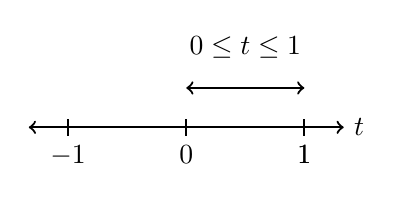
\begin{tikzpicture}

% Draw the line
\draw[thick, <->] (-2,0) -- (2,0) node[right] {$t$};

% Mark and label specific points
\foreach \x/\xtext in {-1.5/$-1$, 0/$0$, 1.5/$1$}
  \draw[thick] (\x,3pt) -- (\x,-3pt) node[below] {\xtext};

% Mark the point 1
\draw[thick] (1.5,3pt) -- (1.5,-3pt) node[below] {$1$};

% Draw the interval of continuity
\draw[thick,<->] (0,0.5) -- (1.5,0.5);
\node at (0.75,0.75) [above] {$0 \leq t \leq 1$};

\end{tikzpicture}
\end{center}

Thus, the largest interval of continuity including \(t = 1\) is \((0, 3)\).



\section*{II.2: Homogeneous Linear Equations}

A homogeneous linear differential equation has the form:
\[
y^{(n)} + a_{n-1}(t)y^{(n-1)} + \dots + a_1(t)y' + a_0(t)y = 0
\]

If \( y_1(t) \) and \( y_2(t) \) are two solutions, then \( c_1 y_1(t) + c_2 y_2(t) \) is also a solution for any constants \( c_1 \) and \( c_2 \).

\textbf{Check:}
\[
\frac{d}{dt}(c_1 y_1 + c_2 y_2) = c_1 y_1' + c_2 y_2'
\]

If \( y_1 \) and \( y_2 \) are solutions, then:
\[
(c_1 y_1 + c_2 y_2)^{(n)} + a_{n-1}(t)(c_1 y_1 + c_2 y_2)^{(n-1)} + \dots + a_1(t)(c_1 y_1 + c_2 y_2)' + a_0(t)(c_1 y_1 + c_2 y_2) = 0
\]

This simplifies to:
\[
c_1 (y_1^{(n)} + a_{n-1} y_1^{(n-1)} + \dots + a_1 y_1' + a_0 y_1) + c_2 (y_2^{(n)} + a_{n-1} y_2^{(n-1)} + \dots + a_1 y_2' + a_0 y_2) = 0
\]

Since \( y_1 \) and \( y_2 \) are solutions:
\[
c_1 \cdot 0 + c_2 \cdot 0 = 0
\]

Thus, \( c_1 y_1 + c_2 y_2 \) is a solution.

\textbf{Example:} We know (i.e., we can check) that \( e^{2t} \) and \( e^{-t} \) are solutions to \( y'' - y' - 2y = 0 \).

Find a solution to the IVP with \( y(0) = 4 \) and \( y'(0) = 2 \).

\textbf{Solution:} We can try to look for a solution of the form:
\[
y = c_1 e^{2t} + c_2 e^{-t}
\]

Then,
\[
y'(t) = 2c_1 e^{2t} - c_2 e^{-t}
\]

Using the initial conditions:
\[
y(0) = c_1 + c_2 = 4
\]
\[
y'(0) = 2c_1 - c_2 = 2
\]

Solving these equations, we get:
\[
c_1 = 2, \quad c_2 = 2
\]

Thus, the solution is:
\[
y = 2e^{2t} + 2e^{-t}
\]

\textbf{Example:} We can check that \( \sin(2t) \) and \( \cos(2t) \) are solutions to \( y'' + 4y = 0 \).

Find a solution to the IVP with \( y(0) = 3 \) and \( y'(0) = -2 \).

\textbf{Solution:} We can try to look for a solution of the form:
\[
y = c_1 \sin(2t) + c_2 \cos(2t)
\]

Then,
\[
y'(t) = 2c_1 \cos(2t) - 2c_2 \sin(2t)
\]

Using the initial conditions:
\[
y(0) = c_2 = 3
\]
\[
y'(0) = 2c_1 = -2 \quad \Rightarrow \quad c_1 = -1
\]

Thus, the solution is:
\[
y = -\sin(2t) + 3\cos(2t)
\]

\textbf{Non-example:} We know that \( e^{-t} \) and \( 2e^{-t} \) are solutions to \( y'' - y' - 2y = 0 \). Solve \( y(0) = 4 \) and \( y'(0) = 2 \).

\textbf{Solution:} We can try to look for a solution of the form:
\[
y = c_1 e^{-t} + c_2 e^{-2t}
\]

Then,
\[
y'(t) = -c_1 e^{-t} - 2c_2 e^{-2t}
\]

Using the initial conditions:
\[
y(0) = c_1 + c_2 = 4
\]
\[
y'(0) = -c_1 - 2c_2 = 2
\]

Solving these equations, we get:
\[
0 \neq 6
\]

Thus, there is no solution.

\textbf{Example:} Solve the IVP \( y'' - y' - 2y = 0 \) with \( y(0) = y_0 \) and \( y'(0) = y_1 \).

\textbf{Solution:} Guess that \( y = c_1 e^{-t} + c_2 e^{-2t} \) solves the ODE.

Using the initial conditions:
\[
 c_1 + c_2 = y_0
\]
\[
2c_1 - c_2 = y_1
\]

Solving these equations simultaneously, we get:
\[
c_1 = \frac{y_1 + y_0}{3}
\]
\[
c_2 = \frac{2y_0 - y_1}{3}
\]

Thus, the solution to the IVP is:
\[
y = \frac{y_1 + y_0}{3} e^{-t} + \frac{2y_0 - y_1}{3} e^{-2t}
\]

\pagebreak

\section*{Lecture 9, Tuesday 9/24/2024}

(Exam 1)

\pagebreak

\section*{Lecture 10, Thursday 9/26/2024}

\subsection*{II.2 Continued: Higher-Order Linear Differential Equations}

\textbf{Example:} Solve the IVP \( y'' - y' - 2y = 0 \) with \( y(0) = y_0 \) and \( y'(0) = y_1 \).

\textbf{Solution:} We have solutions \( y = e^{-t} \) and \( y = e^{-2t} \).

Assume the solution is of the form \( y = c_1 e^{-t} + c_2 e^{-2t} \), where \( c_1 \) and \( c_2 \) are constants.

Using the initial conditions:
\[
y(0) = c_1 + c_2 = y_0
\]
\[
y'(0) = -c_1 - 2c_2 = y_1
\]

Turn this into a matrix equation:
\[
\begin{pmatrix}
1 & 1 \\
-1 & -2
\end{pmatrix}
\begin{pmatrix}
c_1 \\
c_2
\end{pmatrix}
=
\begin{pmatrix}
y_0 \\
y_1
\end{pmatrix}
\]

Solve it using linear algebra.

\subsection*{II.3: Systems of Linear Equations}

A system of linear equations with variables can generally be written in square format with \( n \) equations and \( n \) variables:
\[
\begin{aligned}
a_{11}x_1 + a_{12}x_2 + \cdots + a_{1n}x_n &= b_1 \\
a_{21}x_1 + a_{22}x_2 + \cdots + a_{2n}x_n &= b_2 \\
&\vdots \\
a_{m1}x_m + a_{m2}x_m + \cdots + a_{mn}x_n &= b_n
\end{aligned}
\]
where \( a_{ij} \) are real constants called the coefficients of the system.

If \( b_1 = b_2 = \cdots = b_n = 0 \), the system is homogeneous. If any \( b_i \) is not 0, the system is nonhomogeneous. A solution \( x_1 = x_2 = \cdots = x_n = 0 \) is called the trivial solution.

If there are two solutions \( x_1, \ldots, x_n \) and \( y_{11}, \ldots, y_{1n} \) for a particular nonhomogeneous system, then setting \( z_1 = x_1 - y_{11}, z_2 = x_2 - y_{12}, \ldots, z_n = x_n - y_{1n} \) gives a non-trivial solution of the corresponding homogeneous system:
\[
a_1z_1 + \cdots + a_nz_n = a_{11}x_1 - a_{11}y_{11} + \cdots + a_{1n}x_n - a_{1n}y_{1n} = b_1 - b_1 = 0
\]

\textbf{Upshot:} If a nonhomogeneous system has multiple solutions, the corresponding homogeneous system has a non-trivial solution.

Write the system in matrix form:
\[
A \mathbf{x} = \mathbf{b}
\]
where \( A \) is an \( n \times n \) matrix, and \( \mathbf{x} \) and \( \mathbf{b} \) are \( n \times 1 \) vectors:
\[
\mathbf{x} = \begin{pmatrix}
x_1 \\
\vdots \\
x_n
\end{pmatrix}, \quad
\mathbf{b} = \begin{pmatrix}
b_1 \\
\vdots \\
b_n
\end{pmatrix}, \quad
A = (a_{ij})
\]

\textbf{Idea:} Solve the system by inverting matrix \( A \). Multiply both sides by \( A^{-1} \):
\[
A^{-1} (A \mathbf{x}) = A^{-1} \mathbf{b} \implies I \mathbf{x} = A^{-1} \mathbf{b}
\]

\textbf{Problem:} \( A^{-1} \) doesn't always exist. \( A^{-1} \) exists if and only if \( \det(A) \neq 0 \).

\textbf{Why?} \( \det(I) = 1 \), \( \det(A^{-1}) = \frac{1}{\det(A)} \).

\textbf{Determinants:}
\[
\det(A) = |A|
\]
\[
\begin{vmatrix}
a & b \\
c & d
\end{vmatrix}
= ad - bc
\]
\[
\begin{vmatrix}
a & b & c \\
d & e & f \\
g & h & i
\end{vmatrix}
= aei + bfg + cdh - ceg - bdi - afh
\]

If \( \det(A) \neq 0 \), then there is a unique solution \( \mathbf{x} = A^{-1} \mathbf{b} \).

If \( \det(A) = 0 \), then \( A\mathbf{x} = \mathbf{b} \) might not have a solution, but if it does, it has infinitely many solutions.

For a \( 2 \times 2 \) matrix \( A \), the formula for \( A^{-1} \) is:
\[
A^{-1} = \frac{1}{\det(A)} \begin{pmatrix}
d & -b \\
-c & a
\end{pmatrix}
\]
where \( \det(A) = ad - bc \).

Given the system:
\[
\begin{pmatrix}
1 & 1 \\
2 & -1
\end{pmatrix}
\begin{pmatrix}
c_1 \\
c_2
\end{pmatrix}
=
\begin{pmatrix}
y_0 \\
y_1
\end{pmatrix}
\]

We have \( A\mathbf{x} = \mathbf{b} \).

Calculate the determinant:
\[
\det(A) = 1 \cdot (-1) - 1 \cdot 2 = -1 - 2 = -3
\]

Then, the inverse of \( A \) is:
\[
A^{-1} = \frac{1}{-3} \begin{pmatrix}
-1 & -1 \\
2 & 1
\end{pmatrix}
= \begin{pmatrix}
\frac{1}{3} & \frac{1}{3} \\
-\frac{2}{3} & -\frac{1}{3}
\end{pmatrix}
\]

So,
\[
\begin{pmatrix}
c_1 \\
c_2
\end{pmatrix}
= A^{-1} \mathbf{b} = \frac{1}{-3} \begin{pmatrix}
-1 & -1 \\
2 & 1
\end{pmatrix}
\begin{pmatrix}
y_0 \\
y_1
\end{pmatrix}
= \begin{pmatrix}
\frac{1}{3}(y_1 + y_0) \\
\frac{1}{3}(2y_0 - y_1)
\end{pmatrix}
\]

\subsection*{Wronskians}

Say we have an \( n \)-th order linear ODE with solutions \( Y_1(t), \ldots, Y_n(t) \).

The Wronskian is defined as:
\[
W(t) = \begin{vmatrix}
Y_1(t) & Y_2(t) & \cdots & Y_n(t) \\
Y_1'(t) & Y_2'(t) & \cdots & Y_n'(t) \\
\vdots & \vdots & \ddots & \vdots \\
Y_1^{(n-1)}(t) & Y_2^{(n-1)}(t) & \cdots & Y_n^{(n-1)}(t)
\end{vmatrix}
\]

\textbf{Question:} When is there a solution to the IVP with \( y(t_i) = y_i \), \( y'(t_i) = y_i' \), ..., \( y^{(n-1)}(t_i) = y_i^{(n-1)} \)?

Using initial conditions:
\[
\begin{aligned}
y(t_i) &= y_0 \rightarrow c_1 Y_1(t_i) + c_2 Y_2(t_i) + \cdots + c_n Y_n(t_i) = y_0 \\
y'(t_i) &= y_1 \rightarrow c_1 Y_1'(t_i) + c_2 Y_2'(t_i) + \cdots + c_n Y_n'(t_i) = y_1 \\
&\vdots \\
y^{(n-1)}(t_i) &= y_{n-1} \rightarrow c_1 Y_1^{(n-1)}(t_i) + c_2 Y_2^{(n-1)}(t_i) + \cdots + c_n Y_n^{(n-1)}(t_i) = y_{n-1}
\end{aligned}
\]

This is a system of linear equations for \( c_1, \ldots, c_n \).

Write this system using matrices:
\[
\begin{pmatrix}
Y_1(t_i) & Y_2(t_i) & \cdots & Y_n(t_i) \\
Y_1'(t_i) & Y_2'(t_i) & \cdots & Y_n'(t_i) \\
\vdots & \vdots & \ddots & \vdots \\
Y_1^{(n-1)}(t_i) & Y_2^{(n-1)}(t_i) & \cdots & Y_n^{(n-1)}(t_i)
\end{pmatrix}
\begin{pmatrix}
c_1 \\
c_2 \\
\vdots \\
c_n
\end{pmatrix}
=
\begin{pmatrix}
y_0 \\
y_1 \\
\vdots \\
y_{n-1}
\end{pmatrix}
\]

There is a solution for every choice of \( y_0, \ldots, y_{n-1} \) exactly when \( \det(A) \neq 0 \).

This determinant is called the Wronskian of \( Y_1, \ldots, Y_n \) at \( t_i \):
\[
\text{Wr}(Y_1, \ldots, Y_n)(t_i)
\]

\textbf{Example:} \( Y_1(t) = e^{2t}, Y_2(t) = e^{-t} \)
\[
W(Y_1, Y_2)(0) = \begin{vmatrix}
Y_1(0) & Y_2(0) \\
Y_1'(0) & Y_2'(0)
\end{vmatrix}
= \begin{vmatrix}
1 & 1 \\
2 & -1
\end{vmatrix}
= -3
\]

More generally,
\[
\text{Wr}(Y_1, \ldots, Y_n)(t) = \begin{vmatrix}
e^{2t} & e^{-t} \\
2e^{2t} & -e^{-t}
\end{vmatrix}
= -3e^{t}
\]

Since \( \text{Wr}(e^{2t}, e^{-t})(t) \) is never 0, we have:
\[
y = c_1 e^{2t} + c_2 e^{-t}
\]

\textbf{Solve IVPs:}
\[
\begin{cases}
y'' - y' - 2y = 0 \\
y(t_i) = y_0 \\
y'(t_i) = y_1
\end{cases}
\]

For any \( t_i \) and any \( y_0, y_1 \), we say that \( y = c_1 e^{2t} + c_2 e^{-t} \) is the general solution to \( y'' - y' - 2y = 0 \).

\textbf{Example:} \( Y_1 = e^{-t}, Y_2 = 2e^{-t} \)
\[
\text{Wr}(e^{-t}, 2e^{-t})(t) = \begin{vmatrix}
e^{-t} & 2e^{-t} \\
-e^{-t} & -2e^{-t}
\end{vmatrix}
= -2e^{-2t} + 2e^{-2t} = 0
\]

\( y = c_1 e^{-t} + c_2 e^{-t} \) cannot solve all IVPs.

\textbf{Example:} \( y_1 = \cos(2t), y_2 = \sin(2t) \)
\[
\text{Wr}(\cos(2t), \sin(2t))(t) = \begin{vmatrix}
\cos(2t) & \sin(2t) \\
-2\sin(2t) & 2\cos(2t)
\end{vmatrix}
= 2\cos^2(2t) + 2\sin^2(2t) = 2
\]

Since \( \text{Wr}(y_1, y_2)(t) \) is never 0, we have:
\[
y = c_1 \cos(2t) + c_2 \sin(2t)
\]

This is the general solution to \( y'' + 4y = 0 \).


Theorem: if the coeffcients of a homogeneous linear ODE are continuous on \((a, b)\) and \(Y_1, \ldots, Y_n\) are solutions, then \(\text{Wr}(Y_1, \ldots, Y_n)(t)\) is never 0 on \((a, b)\) or always 0 on \((a, b)\).


\section*{Lecture 11, Tuesday 10/1/2024}

\textbf{Quiz Coverage:} II.1, II.2 (up to \& including 3), II.3.

\textbf{Note:} Thursday's class is prerecorded.

\textbf{Recall:} If $y_1, \ldots, y_n$ are solutions of an $n$th order linear homogeneous ODE, then:

\[
\text{Wr}(y_1, \ldots, y_n)(t) \neq 0
\]

\textbf{Reminder:} The Wronskian is defined as:
\[
\text{Wr}(y_1, \ldots, y_n)(t) = \det 
\begin{pmatrix}
y_1 & \cdots & y_n \\
y_1' & \cdots & y_n' \\
\vdots & \ddots & \vdots \\
y_1^{(n-1)} & \cdots & y_n^{(n-1)}
\end{pmatrix}
\]

Then functions of the form $y = c_1y_1 + \cdots + c_ny_n$ are solutions to every IVP with initial $t$-value $t_0$.

We call such a set of functions $\{y_1, \ldots, y_n\}$ a \textit{fundamental set of solutions} at $t_0$.

And $y = c_1y_1 + \cdots + c_ny_n$ is called the \textit{general solution} to the ODE (at $t_0$).

\textbf{Example:} We saw $y_1 = e^{2t}$, $y_2 = e^{-t}$ are solutions to $y'' - y' - 2y = 0$

and $\text{Wr}(e^{2t}, e^{-t})(t) \neq 0 \Rightarrow \{e^{2t}, e^{-t}\}$ is a fundamental set of solutions at $t$.

And $y = c_1e^{2t} + c_2e^{-t}$ is the general solution at $t$.

\subsection*{Natural Fundamental Sets of Solutions}

Fix an initial $t$-value $t_I$. Consider the ODE:
\[
y^{(n)} + a_{n-1}(t)y^{(n-1)} + \cdots + a_1(t)y' + a_0(t)y = 0
\]

Define $N_k(t)$ for $k = 0, 1, \ldots, n-1$ as the solution to the IVP:

\[
\begin{cases}
y^{(j)}(t_I) = 0 & \text{for } j \neq k \\
y^{(k)}(t_I) = 1
\end{cases}
\]

Explicitly:
\begin{align*}
N_0(t): & \quad y(t_I) = 1, \quad y'(t_I) = 0, \quad \ldots, \quad y^{(n-1)}(t_I) = 0 \\
N_1(t): & \quad y(t_I) = 0, \quad y'(t_I) = 1, \quad \ldots, \quad y^{(n-1)}(t_I) = 0 \\
& \vdots \\
N_{n-1}(t): & \quad y(t_I) = 0, \quad y'(t_I) = 0, \quad \ldots, \quad y^{(n-1)}(t_I) = 1
\end{align*}

Then $\{N_0, N_1, \ldots, N_{n-1}\}$ is a fundamental set of solutions at $t_I$.

Why? 
\begin{align*}
\text{Wr}(N_0, \ldots, N_{n-1})(t_I) &= \det
\begin{pmatrix}
N_0(t_I) & \cdots & N_{n-1}(t_I) \\
N_0'(t_I) & \cdots & N_{n-1}'(t_I) \\
\vdots & \ddots & \vdots \\
N_0^{(n-1)}(t_I) & \cdots & N_{n-1}^{(n-1)}(t_I)
\end{pmatrix} \\
&= \det(I_n) = 1 \neq 0
\end{align*}

This is called the \textit{natural} fundamental set of solutions at $t_I$.

\textbf{Why is this important?} The natural fundamental set of solutions allows us to easily solve initial value problems (IVPs). Consider the IVP:

\[
y^{(n-1)}(t_I) = y_{n-1}, \quad y^{(n-2)}(t_I) = y_{n-2}, \quad \ldots, \quad y'(t_I) = y_1, \quad y(t_I) = y_0
\]

The solution to this IVP is given by:

\[
y(t) = y_0N_0(t) + y_1N_1(t) + \cdots + y_{n-1}N_{n-1}(t)
\]

We can verify that this solution satisfies the initial conditions:

\begin{align*}
y(t_I) &= y_0N_0(t_I) + y_1N_1(t_I) + \cdots + y_{n-1}N_{n-1}(t_I) = y_0 \cdot 1 + y_1 \cdot 0 + \cdots + y_{n-1} \cdot 0 = y_0 \\
y'(t_I) &= y_0N_0'(t_I) + y_1N_1'(t_I) + \cdots + y_{n-1}N_{n-1}'(t_I) = y_0 \cdot 0 + y_1 \cdot 1 + \cdots + y_{n-1} \cdot 0 = y_1 \\
&\vdots \\
y^{(n-1)}(t_I) &= y_0N_0^{(n-1)}(t_I) + y_1N_1^{(n-1)}(t_I) + \cdots + y_{n-1}N_{n-1}^{(n-1)}(t_I) = y_0 \cdot 0 + y_1 \cdot 0 + \cdots + y_{n-1} \cdot 1 = y_{n-1}
\end{align*}
This demonstrates that the natural fundamental set of solutions provides a straightforward method for constructing solutions to IVPs.

\subsection*{Example: Natural Fundamental Set and IVP Solution}

Consider the differential equation $y''+4y = 0$ with solutions $y_1(t) = \cos(2t)$ and $y_2(t) = \sin(2t)$.

\textbf{Task 1:} Find a natural fundamental set of solutions at $t = 0$.

Let $N_0(t) = c_1\cos(2t)$ and $N_1(t) = c_2\sin(2t)$.

For $N_0(t)$:
\begin{align*}
N_0(0) &= 1 \implies c_1\cos(0) = 1 \implies c_1 = 1
\end{align*}

For $N_1(t)$:
\begin{align*}
N_1(0) &= 0 \quad \text{(satisfied automatically)} \\
N_1'(0) &= 1 \implies 2c_2\cos(0) = 1 \implies c_2 = \frac{1}{2}
\end{align*}

Thus, the natural fundamental set of solutions at $t=0$ is:
\begin{align*}
N_0(t) &= \cos(2t) \\
N_1(t) &= \frac{1}{2}\sin(2t)
\end{align*}

\textbf{Task 2:} Solve the following IVP:
\begin{equation*}
\begin{cases}
y''+4y = 0 \\
y(0) = 7 \\
y'(0) = -3
\end{cases}
\end{equation*}

The solution is given by:
\begin{align*}
y(t) &= 7N_0(t) - 3N_1(t) \\
&= 7\cos(2t) - 3\left(\frac{1}{2}\sin(2t)\right) \\
&= 7\cos(2t) - \frac{3}{2}\sin(2t)
\end{align*}

\subsection*{Linear Independence}

A set of functions $\{y_1, \ldots, y_n\}$ is linearly independent on an interval $(a,b)$ if:
\begin{equation*}
c_1y_1(t) + \cdots + c_ny_n(t) = 0 \quad \text{for all } t \in (a,b)
\end{equation*}
implies $c_1 = \cdots = c_n = 0$.

\textbf{Non-example:} Consider $y_1 = e^{-t}$ and $y_2 = 2e^{-t}$. Then:
\begin{equation*}
2y_1 - y_2 = 2e^{-t} - 2e^{-t} = 0
\end{equation*}
Therefore, $y_1$ and $y_2$ are linearly dependent.

\textbf{Theorem 1:} If $\text{Wr}(y_1, \ldots, y_n)(t) \neq 0$ on $(a,b)$, then $y_1, \ldots, y_n$ are linearly independent on $(a,b)$.

\textbf{Theorem 2:} If $\text{Wr}(y_1, \ldots, y_n)(t) = 0$ on $(a,b)$, then $y_1, \ldots, y_n$ are linearly dependent on $(a,b)$.

\subsection*{II.4: Homogeneous Linear ODEs with Constant Coefficients}

The general form of a homogeneous linear ODE with constant coefficients is:
\begin{equation*}
y^{(n)} + a_{n-1}y^{(n-1)} + \cdots + a_1y' + a_0y = 0
\end{equation*}
where $a_0, \ldots, a_{n-1}$ are constants.

\textbf{Example:} Consider the equation $y'' - y' - 2y = 0$

We have already seen that $y = e^{2t}$ and $y = e^{-t}$ are solutions.

Let's guess that our solutions are of the form $y = e^{zt}$. Then:
\begin{align*}
y &= e^{zt} \\
y' &= ze^{zt} \\
y'' &= z^2e^{zt}
\end{align*}

Substituting into the original equation:
\begin{equation*}
z^2e^{zt} - ze^{zt} - 2e^{zt} = 0
\end{equation*}

Dividing by $e^{zt}$:
\begin{equation*}
z^2 - z - 2 = 0
\end{equation*}

Solving this quadratic equation:
\begin{equation*}
z = 2 \text{ or } z = -1
\end{equation*}

Therefore, we have solutions $y = e^{2t}$ and $y = e^{-t}$.

In general, for a linear ODE with constant coefficients, we can use the characteristic polynomial to find the solutions.

If we plug $y=e^{zt}$ into our ODE, we get (remembering $\frac{d^k}{dt^k} e^{zt} = z^k e^{zt}$):
\begin{equation*}
z^n e^{zt} + a_1 z^{n-1} e^{zt} + \cdots + a_n e^{zt} = 0
\end{equation*}

Factoring out $e^{zt}$:
\begin{equation*}
(z^n + a_1 z^{n-1} + \cdots + a_n) e^{zt} = 0
\end{equation*}

This gives us the characteristic polynomial:
\[
p(z) = z^n + a_1 z^{n-1} + \cdots + a_n
\]

Therefore, if $z$ is any root of $p(z) = 0$, then $y = e^{zt}$ is a solution to our ODE.

\textbf{Note:} An $n$th order ODE corresponds to an $n$th degree polynomial, which has the potential to have $n$ roots.

\textbf{Problem:} $p(z) = 0$ may have repeated roots or complex roots.

\textbf{Easier case:} Simple (non-repeated) real roots

In this case, we can factor $p(z)$ as:
\[
p(z) = (z-r_1)(z-r_2) \cdots (z-r_n)
\]
where $r_1, \ldots, r_n$ are distinct real numbers.

\textbf{Consequence:} $e^{r_1t}, \ldots, e^{r_nt}$ are solutions

It turns out that $\text{Wr}(e^{r_1t}, \ldots, e^{r_nt})(t) \neq 0$

We can verify this by computing the Wronskian:
\[
\text{Wr}(e^{r_1t}, \ldots, e^{r_nt})(t) = 
\begin{vmatrix}
e^{r_1t} & e^{r_2t} & \cdots & e^{r_nt} \\
r_1e^{r_1t} & r_2e^{r_2t} & \cdots & r_ne^{r_nt} \\
\vdots & \vdots & \ddots & \vdots \\
r_1^{n-1}e^{r_1t} & r_2^{n-1}e^{r_2t} & \cdots & r_n^{n-1}e^{r_nt}
\end{vmatrix}
\]

For $n = 2$, we have:
\[
\begin{vmatrix}
e^{r_1t} & e^{r_2t} \\
r_1e^{r_1t} & r_2e^{r_2t}
\end{vmatrix} = e^{(r_1+r_2)t}(r_2 - r_1) \neq 0
\]

since $r_2 \neq r_1$ and $e^{(r_1+r_2)t} > 0$ for all $t$.

Hence, $\{e^{r_1t}, \ldots, e^{r_nt}\}$ is a fundamental set of solutions, and the general solution is:

\[
y = c_1e^{r_1t} + \cdots + c_ne^{r_nt}
\]

\textbf{Example 1:} Solve $y''+7y'+12y = 0$.

Solution:
\begin{align*}
p(z) &= z^2+7z+12 \\
     &= (z+3)(z+4)
\end{align*}

The roots are $r_1 = -3$ and $r_2 = -4$. Therefore, $e^{-3t}$ and $e^{-4t}$ are solutions.

The general solution is:
\[
y = c_1e^{-4t} + c_2e^{-3t}
\]

\textbf{Example 2:} Solve $y''-2y'-y = 0$.
Solution:
\begin{align*}
p(z) &= z^2-2z-1 \\
     &= (z-(1+\sqrt{2}))(z-(1-\sqrt{2}))
\end{align*}

The characteristic equation has two distinct real roots:
\[
r_1 = 1+\sqrt{2} \quad \text{and} \quad r_2 = 1-\sqrt{2}
\]

Therefore, the general solution is:

\[
y = c_1e^{r_1t} + c_2e^{r_2t} = c_1e^{(1+\sqrt{2})t} + c_2e^{(1-\sqrt{2})t}
\]

where $c_1$ and $c_2$ are arbitrary constants.

\textbf{Example 3:} Solve $y''' + 2y'' - y' - 2y = 0$.

\textbf{Solution:}
Let's find the characteristic equation and its roots:

\begin{align*}
p(z) &= z^3 + 2z^2 - z - 2 \\
     &= (z+2)(z+1)(z-1)
\end{align*}

To find the roots, we can use the Rational Root Theorem:

\textit{Theorem:} If $p(z) = a_nz^n + \cdots + a_1z + a_0$ is a polynomial with integer coefficients, then any rational root of $p(z) = 0$ is of the form $\pm \frac{p}{q}$, where $p$ is a factor of $a_0$ and $q$ is a factor of $a_n$.

In our case, $a_0 = -2$ and $a_3 = 1$. The possible rational roots are $\pm 1, \pm 2$.

Testing these values, we find the roots:

\[
r_1 = -2, \quad r_2 = -1, \quad r_3 = 1
\]

Therefore, the general solution is:

\[
y = c_1e^{-2t} + c_2e^{-t} + c_3e^t
\]

where $c_1$, $c_2$, and $c_3$ are arbitrary constants.

\section*{Lecture 12, Thursday 10/3/2024}

\subsection*{II.4 Continued: Real Roots with Multiplicity}

\textbf{Recall:} For a linear homogeneous ODE of order $n$:
\[
y^{(n)} + a_{n-1}y^{(n-1)} + \cdots + a_1y' + a_0y = 0
\]
The characteristic polynomial is:
\[
p(z) = z^n + a_{n-1}z^{n-1} + \cdots + a_1z + a_0
\]

\textbf{Key Points:}
\begin{itemize}
    \item If $r$ is a real root of $p(z)$, then $e^{rt}$ is a solution to the ODE.
    \item For real roots with multiplicity $k > 1$:
    \begin{itemize}
        \item $(z-r)$ appears $k$ times in the factorization of $p(z)$
        \item If $p(z) = (z-r)^k q(z)$, then $e^{rt}, te^{rt}, t^2e^{rt}, \ldots, t^{k-1}e^{rt}$ are solutions to the ODE.
    \end{itemize}
\end{itemize}

\textbf{Example:} Solve $y''' + 2y'' + y' = 0$

\textbf{Solution:}
\begin{enumerate}
    \item Characteristic polynomial: $p(z) = z^3 + 2z^2 + z$
    \item Factor $p(z)$: $z(z+1)^2 = 0$
    \item Roots: $z = 0$ (multiplicity 1), $z = -1$ (multiplicity 2)
    \item Solutions: $e^{0t} = 1$, $e^{-t}$, $te^{-t}$
    \item General solution: $y = c_1 + c_2e^{-t} + c_3te^{-t}$
\end{enumerate}

\textbf{Theorem:} $e^{rt}, te^{rt}, \ldots, t^{k-1}e^{rt}$ are linearly independent.

\textbf{Proof sketch for $k=2$:}
Calculate the Wronskian:
\[
\text{Wr}(e^{rt}, te^{rt})(t) = \begin{vmatrix}
e^{rt} & te^{rt} \\
re^{rt} & e^{rt} + rte^{rt}
\end{vmatrix} = e^{2rt} \neq 0
\]

\textbf{Why this works:}
When we substitute $y = e^{zt}$ into the ODE, we get $p(z)e^{zt} = 0$.
This is because:
\[
\frac{d^k}{dt^k} (e^{zt}) = z^k e^{zt}
\]

Note: $te^{zt} = \frac{\partial}{\partial z}(e^{zt})$

So:
\begin{align*}
\frac{d^k}{dt^k}(te^{zt}) &= z^k e^{zt} + k z^{k-1} e^{zt} \\
&= e^{zt}(tz^k + k z^{k-1})
\end{align*}

Plugging $te^{zt}$ into the ODE, we get:
\[
p'(z) + tp(z)e^{zt}
\]
This is called a key identity.

\textbf{Fact:} $r$ is a double root of $p(z)$ if and only if $p(z) = (z-r)^2 q(z)$ for some polynomial $q(z)$.

In this case, $p(r) = 0$ and $p'(r) = 0$.

If $r$ is a double root, then plugging $z = r$ into the key identity shows that $te^{rt}$ is a solution:
\[
(p'(r) + tp(r))e^{rt} = 0 \implies te^{rt} \text{ is a solution}
\]

Similarly, plugging $t^2e^{rt}$ into the ODE gives:
\[
(p''(r) + 2tp'(r) + t^2p(r))e^{rt} = 0 \implies t^2e^{rt} \text{ is a solution}
\]

\textbf{Example:} Solve $y^{(7)} - 6y^{(5)} + 9y^{(3)} = 0$

\textbf{Solution:} 
Characteristic polynomial: $p(z) = z^7 - 6z^5 + 9z^3 = z^3(z^2-3)^2$

Roots:
\begin{itemize}
    \item $z = 0$ (multiplicity 3)
    \item $z = \sqrt{3}$ (multiplicity 2)
    \item $z = -\sqrt{3}$ (multiplicity 2)
\end{itemize}

Solutions: $1, t, t^2, e^{\sqrt{3}t}, te^{\sqrt{3}t}, e^{-\sqrt{3}t}, te^{-\sqrt{3}t}$

General solution:
\[
y = c_1 + c_2t + c_3t^2 + c_4e^{\sqrt{3}t} + c_5te^{\sqrt{3}t} + c_6e^{-\sqrt{3}t} + c_7te^{-\sqrt{3}t}
\]

\subsection*{Complex Roots}

\textbf{Example:} Solve $y'' + 2y' + 2y = 0$

\textbf{Solution:} 
Characteristic polynomial: $p(z) = z^2 + 2z + 2$

Roots: $z = -1 \pm i$

For complex roots, we use Euler's identity: $e^{i\theta} = \cos\theta + i\sin\theta$

In general, for a complex root $r + si$:
\[
e^{(r+si)t} = e^{rt}(\cos(st) + i\sin(st)) = e^{rt}\cos(st) + ie^{rt}\sin(st)
\]
Whenever we have a root $r + si$ of $p(z)$, we also get the conjugate root $r - si$.
\subsection*{Complex Roots}

For complex roots $r \pm si$, we use the following properties:

\begin{align*}
\cos(-x) &= \cos(x) \\
\sin(-x) &= -\sin(x)
\end{align*}

This leads to two linearly independent solutions:
\begin{align*}
e^{rt}\cos(st) &\text{ is a solution} \\
e^{rt}\sin(st) &\text{ is a solution}
\end{align*}

\textbf{Upshot:} When $r \pm si$ is a root of the characteristic polynomial, we get two solutions: $e^{rt}\cos(st)$ and $e^{rt}\sin(st)$.

\textbf{Example 1:} Solve $y'' + 2y' + 2y = 0$

\textbf{Solution:} 
The characteristic polynomial $p(z) = z^2 + 2z + 2$ has roots $-1 \pm i$.
Therefore, the solutions are $e^{-t}\cos(t)$ and $e^{-t}\sin(t)$.

General solution: $y = c_1e^{-t}\cos(t) + c_2e^{-t}\sin(t)$

\textbf{Example 2:} Solve $y''+4y=0$

\textbf{Solution:} 
Characteristic polynomial: $p(z) = z^2 + 4$
Roots: $z = \pm 2i$
Solutions: $e^{2it}$, $e^{-2it}$

General solution: $y = c_1\cos(2t) + c_2\sin(2t)$

\textbf{Example 3:} Find the general solution of $(D+5)^3(D^2+4D+5)(D^2+4)y = 0$, where $D = \frac{d}{dt}$

\textbf{Solution:}
Characteristic polynomial: $(z+5)^3(z^2+4z+5)(z^2+4) = 0$

Roots:
\begin{itemize}
    \item $z = -5$ (multiplicity 3)
    \item $z = -2 \pm i$ (multiplicity 1)
    \item $z = \pm 2i$ (multiplicity 1)
\end{itemize}

Solutions:
\begin{itemize}
    \item $e^{-5t}$, $te^{-5t}$, $t^2e^{-5t}$
    \item $e^{-2t}\cos(t)$, $e^{-2t}\sin(t)$
    \item $\cos(2t)$, $\sin(2t)$
\end{itemize}

General solution:
\[
y = c_1e^{-5t} + c_2te^{-5t} + c_3t^2e^{-5t} + c_4e^{-2t}\cos(t) + c_5e^{-2t}\sin(t) + c_6\cos(2t) + c_7\sin(2t)
\]

\subsection*{Complex Roots with Multiplicity > 1}

If $r \pm si$ is a root of $p(z)$ with multiplicity $k > 1$, then the solutions are:
\[
\begin{aligned}
&e^{rt}\cos(st), \quad te^{rt}\cos(st), \quad \ldots, \quad t^{k-1}e^{rt}\cos(st) \\
&e^{rt}\sin(st), \quad te^{rt}\sin(st), \quad \ldots, \quad t^{k-1}e^{rt}\sin(st)
\end{aligned}
\]

\textbf{Example 4:} Solve $y^{(4)} + 4y'' + 4y = 0$

\textbf{Solution:}
\begin{itemize}
    \item Characteristic polynomial: $p(z) = z^4 + 4z^2 + 4 = (z^2+2)^2 = 0$
    \item Roots: $z = \pm i\sqrt{2}$ (multiplicity 2)
    \item Solutions: $\cos(\sqrt{2}t)$, $t\cos(\sqrt{2}t)$, $\sin(\sqrt{2}t)$, $t\sin(\sqrt{2}t)$
\end{itemize}

General solution:
\[
y = c_1\cos(\sqrt{2}t) + c_2t\cos(\sqrt{2}t) + c_3\sin(\sqrt{2}t) + c_4t\sin(\sqrt{2}t)
\]

\textbf{Example 5:} Solve $(D^3-2D^2)(D^2-2D+10)^3(D^2+4D+29)y = 0$

\textbf{Solution:}
\begin{itemize}
    \item Characteristic polynomial: $(z^3-2z^2)(z^2-2z+10)^3(z^2+4z+29) = 0$
    \item Roots:
    \begin{itemize}
        \item $z = 0$ (multiplicity 2)
        \item $z = 2$ (multiplicity 1)
        \item $z = 1 \pm 3i$ (multiplicity 3)
        \item $z = -2 \pm 5i$ (multiplicity 1)
    \end{itemize}
    \item Solutions:
    \begin{itemize}
        \item $1$, $t$
        \item $e^{2t}$
        \item $e^t\cos(3t)$, $e^t\sin(3t)$, $te^t\cos(3t)$, $te^t\sin(3t)$, $t^2e^t\cos(3t)$, $t^2e^t\sin(3t)$
        \item $e^{-2t}\cos(5t)$, $e^{-2t}\sin(5t)$
    \end{itemize}
\end{itemize}

General solution:
\begin{align*}
y = &c_1 + c_2t + c_3e^{2t} \\
&+ (c_4 + c_5t + c_6t^2)e^t\cos(3t) + (c_7 + c_8t + c_9t^2)e^t\sin(3t) \\
&+ c_{10}e^{-2t}\cos(5t) + c_{11}e^{-2t}\sin(5t)
\end{align*}

\section*{Lecture 13, Tuesday 10/8/2024}

\subsection*{II.5: Nonhomogeneous Equations}

Consider the linear differential equation:
\[
L(y) = y^{(n)} + a_{n-1}y^{(n-1)} + \cdots + a_1y' + a_0y = f(t)
\]

The linearity of this equation implies:
\[
L(c_1y_1 + \cdots + c_my_m) = c_1L(y_1) + \cdots + c_mL(y_m)
\]

\textbf{Key Property:} If $Y_1(t)$ and $Y_2(t)$ are two solutions to $L(y) = f(t)$, then $Y_1(t) - Y_2(t)$ is a solution to the homogeneous ODE $L(y) = 0$.

\textbf{Proof:}
\[
L(Y_1 - Y_2) = L(Y_1) - L(Y_2) = f(t) - f(t) = 0
\]

\textbf{Consequence:} If $Y_p(t)$ is a particular solution to $L(y) = f(t)$, then every solution to $L(y) = f(t)$ is of the form $Y_p(t) + y_H(t)$, where $y_H(t)$ is a solution to the homogeneous equation $L(y) = 0$.

\textbf{Process for solving $L(y) = f(t)$:}
\begin{enumerate}
    \item Find the general solution $Y_H(t)$ of the associated homogeneous ODE $L(y) = 0$
    \item Find any particular solution $Y_p(t)$ to $L(y) = f(t)$
    \item The general solution to $L(y) = f(t)$ is $y = Y_H(t) + Y_p(t)$
\end{enumerate}

\textbf{Example:} Find the general solution to $y''+4y = t$, given that $y = \frac{t}{4}$ is one solution.

\textbf{Solution:}
\begin{enumerate}
    \item Homogeneous solution $y_H(t)$:
    \begin{align*}
        z^2+4 &= 0 \\
        z &= \pm 2i \\
        y_H(t) &= c_1\cos(2t) + c_2\sin(2t)
    \end{align*}

    \item Particular solution: $y_p(t) = \frac{t}{4}$

    \item General solution:
    \[
    y = c_1\cos(2t) + c_2\sin(2t) + \frac{t}{4}
    \]
\end{enumerate}

Note: $Y_p(t) = \frac{t}{4} + 2\cos(2t)$ is also a valid particular solution.

\subsection*{Solving Initial Value Problems (IVPs)}

To solve an IVP for a nonhomogeneous linear ODE:
\begin{enumerate}
    \item Find the general solution to $L(y) = f(t)$
    \item Use the initial conditions to solve for the constants $c_1, c_2, \ldots$
\end{enumerate}

\textbf{Example:} Solve the IVP $y''+4y = t$, with $y(0) = 3$ and $y'(0) = -1$

\textbf{Solution:}
\begin{enumerate}
    \item General solution: $y = c_1\cos(2t) + c_2\sin(2t) + \frac{t}{4}$
    \item Apply initial conditions:
    \begin{align*}
        y(0) &= 3: \quad c_1 = 3 \\
        y'(t) &= -2c_1\sin(2t) + 2c_2\cos(2t) + \frac{1}{4} \\
        y'(0) &= -1: \quad 2c_2 + \frac{1}{4} = -1 \implies c_2 = -\frac{5}{8}
    \end{align*}
\end{enumerate}

Therefore, the solution to the IVP is:
\[
y = 3\cos(2t) - \frac{5}{8}\sin(2t) + \frac{t}{4}
\]

\subsection*{II.6: Nonhomogeneous Linear ODEs with Constant Coefficients}

Consider the general form:
\[
L(y) = y^{(n)} + a_{n-1}y^{(n-1)} + \cdots + a_1y' + a_0y = f(t)
\]

where $f(t)$ is of the form:
\[
f(t) = (\alpha_dt^d + \cdots + \alpha_0) e^{rt} \cos(st) + (\beta_dt^d + \cdots + \beta_0) e^{rt} \sin(st)
\]

\textbf{Key terms:}
\begin{itemize}
    \item $d$: degree of $f(t)$
    \item $r + si$: characteristic of $f(t)$
    \item $m$: multiplicity of $r + si$ as a root of $p(z)$, where $p(z)$ is the characteristic polynomial of $L(y)$
    \item Note: $m = 0$ if $p(r+si) \neq 0$
\end{itemize}

\subsection*{Method of Undetermined Coefficients}

\textbf{General Approach:}
\begin{enumerate}
    \item Guess the form of $Y_p(t)$ based on $f(t)$
    \item Calculate $Y_p', Y_p'', \ldots, Y_p^{(n)}$
    \item Substitute into the ODE
    \item Collect terms and equate coefficients
    \item Solve for undetermined coefficients
\end{enumerate}

\textbf{Guessing $Y_p(t)$:}
\begin{itemize}
    \item If $f(t) = (\text{polynomial})e^{rt}$, guess $Y_p(t) = (\text{polynomial of same degree})t^m e^{rt}$
    \item If $f(t) = \alpha e^{rt} \cos(st) + \beta e^{rt} \sin(st)$, guess $Y_p(t) = At^m e^{rt} \cos(st) + Bt^m e^{rt} \sin(st)$
\end{itemize}

\textbf{Example 1:} Find $Y_p(t)$ for $y'' + 2y' + 10y = 6e^{2t}$

\textbf{Solution:}
\begin{itemize}
    \item $d = 0$, $r = 2$, $s = 0$
    \item $p(z) = z^2 + 2z + 10$, roots: $z = -1 \pm 3i$
    \item $m = 0$ (2 is not a root)
    \item Guess: $Y_p(t) = Ae^{2t}$
\end{itemize}

Substituting into the ODE:
\[
(4A + 4A + 10A)e^{2t} = 6e^{2t} \implies 18A = 6 \implies A = \frac{1}{3}
\]

Therefore, $Y_p(t) = \frac{1}{3}e^{2t}$

\textbf{Example 2:} Find $Y_p(t)$ for $y'' - 6y' + 9y = 4te^{3t}$

\textbf{Solution:}
\begin{itemize}
    \item $d = 1$, $r = 3$, $s = 0$
    \item $p(z) = z^2 - 6z + 9 = (z - 3)^2$
    \item $m = 2$
    \item Guess: $Y_p(t) = (At + B)t^2e^{3t} = (At^3 + Bt^2)e^{3t}$
\end{itemize}

Substituting into the ODE and equating coefficients:
\[
6A = 4, \quad 2B = 0 \implies A = \frac{2}{3}, \quad B = 0
\]

Therefore, $Y_p(t) = \frac{2}{3}t^3e^{3t}$

\textbf{Example 3:} Find $Y_p(t)$ for $y'' + 2y' + 10y = \cos(2t)$

\textbf{Solution:}
\begin{itemize}
    \item $d = 0$, $r = 0$, $s = 2$
    \item $p(z) = z^2 + 2z + 10$, roots: $z = -1 \pm 3i$
    \item $m = 0$
    \item Guess: $Y_p(t) = A \cos(2t) + B \sin(2t)$
\end{itemize}

Substituting into the ODE and equating coefficients:
\[
\begin{cases}
6A + 4B = 1 \\
6B - 4A = 0
\end{cases}
\implies A = \frac{1}{13}, \quad B = \frac{3}{26}
\]

Therefore, $Y_p(t) = \frac{1}{13} \cos(2t) + \frac{3}{26} \sin(2t)$

\section*{Lecture 14, Thursday 10/10/2024}

\subsection*{II.6 Continued}

\textbf{Example:} Solve $y''+2y'+10y = 5e^{-t}\sin(3t)$. Find a particular solution.

\textbf{Solution:}

Characteristic polynomial: $p(z) = z^2+2z+10$
Roots: $-1 \pm 3i$

For $f(t) = 5e^{-t}\sin(3t)$, we have $r + si = -1 + 3i$, $d = 0$, $m = 1$

Guess: $Y_p(t) = At e^{-t}\sin(3t) + Bt e^{-t}\cos(3t)$

Substituting $Y_p(t)$, $Y_p'(t)$, and $Y_p''(t)$ into the ODE and simplifying:

\[6Be^{-t}\cos(3t) + 6Ae^{-t}\sin(3t) = 5e^{-t}\sin(3t)\]

Equating coefficients:
\begin{align*}
6B &= 0 \\
-6A &= 5
\end{align*}

Solving: $B = 0$, $A = -\frac{5}{6}$

Therefore, $Y_p(t) = -\frac{5}{6}te^{-t}\sin(3t)$

The general solution is $y = Y_H(t) + Y_p(t)$:

\[y = c_1e^{-t}\cos(3t) + c_2e^{-t}\sin(3t) - \frac{5}{6}te^{-t}\sin(3t)\]

\textbf{Example:} Find the form of a particular solution to $y''+4y = t\cos(2t)$. Do not solve for any constants.

\textbf{Solution:} 
Characteristic equation: $z^2+4 = 0$, roots: $z = \pm 2i$

For $f(t) = t\cos(2t)$, we have $r + si = 0 + 2i$, $d = 1$, $m = 1$

Guess: $Y_p(t) = (A_1t^2 + A_0t)\cos(2t) + (B_1t^2 + B_0t)\sin(2t)$

\textbf{Example:} Solve $L(y) = f(t)$ where $f(t) = e^{2t}+9\cos(5t)$

\textbf{Approach:} Find $Y_{p1}(t)$ for $L(y) = e^{2t}$ and $Y_{p2}(t)$ for $L(y) = 9\cos(5t)$ separately and add them together.

Set $Y_p(t) = Y_{p1}(t) + Y_{p2}(t)$

Because $L(Y_p(t)) = L(Y_{p1}(t)) + L(Y_{p2}(t))$, we have $L(Y_p(t)) = e^{2t} + 9\cos(5t)$

\subsection*{Alternative Approach: Key Identities}

Remember: $L(e^{zt}) = p(z)e^{zt}$

Taking $\frac{d}{dz}$ of both sides:

\begin{align*}
\frac{d}{dz}(L(e^{zt})) &= \frac{d}{dz}(p(z)e^{zt}) = L(te^{zt}) \\
\frac{d}{dz}(p(z)e^{zt}) &= p'(z)e^{zt}+p(z)te^{zt} \\
L(te^{zt}) &= p'(z)e^{zt}+p(z)te^{zt}
\end{align*}

Continuing this process:

\begin{align*}
L(t^2e^{zt}) &= (2p'(z)+p(z)t)te^{zt}+(p'(z)+p(z)t)e^{zt} \\
L(t^3e^{zt}) &= (6p'(z)+p(z)t)te^{zt}+(3p'(z)+p(z)t)e^{zt}
\end{align*}

\textbf{Example:} Solve $y'' - 6y' + 9y = 4te^{3t}$. Find $Y_p(t)$.

\textbf{Solution:} 
Characteristic polynomial: $z^2-6z+9 = (z-3)^2$

$r + si = 3 + 0i$, $d = 1$, $m = 2$

Guess: $Y_p(t) = (A_1t + A_0)t^2e^{3t}$

Using the key identities:

\begin{align*}
L(e^{3t}) &= p(3)e^{3t} = (9-18+9)e^{3t} = 0 \\
L(te^{3t}) &= (2p'(3)+p(3))e^{3t} = 0 \\
L(t^2e^{3t}) &= (6p'(3)+p(3))e^{3t} = 2e^{3t} \\
L(t^3e^{3t}) &= (24p'(3)+6p(3))e^{3t} = 6e^{3t}
\end{align*}

To get $f(t) = 4te^{3t}$:

\[L(\frac{2}{3}t^3e^{3t}) = (\frac{24}{3}p'(3)+\frac{6}{3}p(3))e^{3t} = 4te^{3t}\]

Therefore, $Y_p(t) = \frac{2}{3}t^3e^{3t}$

\subsection*{Examples}

\subsubsection*{Example 1: $y''+2y'+10y = 6e^{2t}$}

\textbf{Solution:} 
\begin{itemize}
    \item Characteristic polynomial: $p(z) = z^2+2z+10$
    \item Roots: $r+si = 2+0i$, $d = 0$, $m = 0$
    \item $f(t) = 6e^{2t}$, $r = 2$
\end{itemize}

Using the key identity:
\begin{align*}
L(e^{2t}) &= p(2)e^{2t} = (4+4+10)e^{2t} = 18e^{2t}
\end{align*}

Hence, $L(\frac{1}{3}e^{2t}) = 6e^{2t}$

Therefore, $Y_p(t) = \frac{1}{3}e^{2t}$

\subsubsection*{Example 2: $y''+2y'+10y = 6te^{2t}$}

\textbf{Solution:} 
\begin{itemize}
    \item Characteristic polynomial: $p(z) = z^2+2z+10$
    \item Roots: $r+si = 2+0i$, $d = 1$, $m = 1$
    \item $f(t) = 6te^{2t}$, $r = 2$
\end{itemize}

Using the key identities:
\begin{align*}
L(e^{2t}) &= p(2)e^{2t} = 18e^{2t} \\
L(te^{2t}) &= (2p'(2)+p(2))e^{2t} = (6+18)e^{2t} = 24e^{2t} \\
L(t^2e^{2t}) &= (6p'(2)+p(2))e^{2t} = 18e^{2t}
\end{align*}

We find that:
\begin{align*}
L(te^{2t}-\frac{1}{3}e^{2t}) &= 18te^{2t} \\
\Rightarrow L(\frac{1}{3}(te^{2t}-\frac{1}{3}e^{2t})) &= 6te^{2t}
\end{align*}

Therefore, $Y_p(t) = \frac{1}{3}(te^{2t}-\frac{1}{3}e^{2t})$

\subsubsection*{Example 3: $y''+2y'+10y = \cos(2t)$}

\textbf{Solution:} 
\begin{itemize}
    \item Characteristic polynomial: $p(z) = z^2+2z+10$
    \item Roots: $r+si = 0+2i$, $d = 0$, $m = 0$
    \item $f(t) = \cos(2t)$, $r = 0$, $s = 2$
\end{itemize}

Using the key identity:
\begin{align*}
L(e^{2it}) &= p(2i)e^{2it} = (6+4i)(\cos(2t)+i\sin(2t)) \\
           &= (6\cos(2t)-4\sin(2t)) + i(6\sin(2t)+4\cos(2t))
\end{align*}

Cancelling out $\sin(2t)$:
\begin{align*}
L(6\cos(2t)+4\sin(2t)) &= (36+16)\cos(2t) = 52\cos(2t)
\end{align*}

Therefore, $Y_p(t) = \frac{1}{52}(6\cos(2t)+4\sin(2t))$

\subsection*{II.7: Variable Coefficients}

\subsubsection*{Reduction of Order}

Consider the equation: $y''+a_1(t)y'+a_0(t)y = 0$

Given $y_1(t)$ is a solution, we guess another solution of the form $y = u(t)y_1(t)$

Differentiating:
\begin{align*}
y' &= u'y_1+uy_1' \\
y'' &= u''y_1+2u'y_1'+uy_1''
\end{align*}

Substituting into the ODE:
\begin{align*}
u''y_1+u'(2y_1'+a_1y_1)+u(y_1''+a_1y_1'+a_0y_1) &= 0
\end{align*}

Let $w = u'$, then:
\begin{align*}
w'y_1+w(2y_1'+a_1y_1)+u(y_1''+a_1y_1'+a_0y_1) &= 0
\end{align*}

This is a separable first-order ODE for $w$. Solve for $w$, then integrate to get $u$.

\subsubsection*{Example: $t^2y-t(t+2)y'+(t+2)y = 0$}

Given $y_1(t)$ is a solution for $t > 0$, find the general solution.

\textbf{Solution:} 
Guess $y = ut$, so $y' = u't+u$, $y'' = u''t+2u'$

Substituting into the ODE:
\begin{align*}
t^3u''-t^3u' &= 0
\end{align*}

As $t > 0$, $u''-u' = 0$

Let $w = u'$, then $w'-w = 0$ or $w' = w$
We see that $w = ce^t$

Therefore, $u' = ce^t$, so $u = ce^t+D$

Our general solution is $y = ut = cte^t+Dt$

\section*{Lecture 15, Tuesday 10/15/2024}

\subsection*{II.7 Continued}

\subsubsection*{Variation of Parameters}

Consider the non-homogeneous equation:
\[
y'' + a_1(t)y' + a_0(t)y = f(t)
\]

Given that the general solution to the homogeneous equation is $y = c_1y_1 + c_2y_2$, we seek a particular solution $Y_p(t)$.

We guess a solution of the form:
\[
Y_p(t) = u_1(t)y_1(t) + u_2(t)y_2(t)
\]

where $u_1(t)$ and $u_2(t)$ are functions to be determined.

Differentiating:
\begin{align*}
Y_p' &= u_1'y_1 + u_1y_1' + u_2'y_2 + u_2y_2' \\
Y_p'' &= u_1''y_1 + 2u_1'y_1' + u_1y_1'' + u_2''y_2 + 2u_2'y_2' + u_2y_2''
\end{align*}

We impose the condition:
\[
u_1'y_1 + u_2'y_2 = 0
\]

This simplifies our expressions to:
\begin{align*}
Y_p' &= u_1y_1' + u_2y_2' \\
Y_p'' &= u_1y_1'' + u_2y_2''
\end{align*}

Substituting into the original ODE:
\[
u_1''y_1 + u_2''y_2 = f(t)
\]

Thus, $u_1$ and $u_2$ must satisfy:
\begin{align*}
u_1'y_1 + u_2'y_2 &= 0 \\
u_1'y_1' + u_2'y_2' &= f(t)
\end{align*}

This system can be written in matrix form:
\[
\begin{pmatrix}
y_1 & y_2 \\
y_1' & y_2'
\end{pmatrix}
\begin{pmatrix}
u_1' \\
u_2'
\end{pmatrix} =
\begin{pmatrix}
0 \\
f(t)
\end{pmatrix}
\]

The determinant of the coefficient matrix is the Wronskian $W(y_1, y_2) = y_1y_2' - y_1'y_2 \neq 0$, as $y_1$ and $y_2$ are linearly independent.

Solving this system:
\[
\begin{pmatrix}
u_1' \\
u_2'
\end{pmatrix} =
\frac{1}{W(y_1, y_2)}
\begin{pmatrix}
y_2 & -y_1 \\
-y_2' & y_1'
\end{pmatrix}
\begin{pmatrix}
0 \\
f(t)
\end{pmatrix}
\]

Therefore:
\[
u_1' = \frac{f(t)y_2}{W}, \quad u_2' = -\frac{f(t)y_1}{W}
\]

Integrating gives us $u_1$ and $u_2$.

\textbf{Example:} Find a general solution of $y'' + y = \sec(t)$

\textbf{Solution:} 
The homogeneous solution $Y_H$ comes from $p(z) = z^2 + 1$, with roots $z = \pm i$:
\[
Y_H = c_1\cos(t) + c_2\sin(t)
\]

We guess a particular solution of the form:
\[
Y_p = u_1\cos(t) + u_2\sin(t)
\]

Using variation of parameters:
\begin{align*}
\cos(t)u_1' + \sin(t)u_2' &= 0 \\
-\sin(t)u_1' + \cos(t)u_2' &= \sec(t)
\end{align*}

Solving this system:
\[
\begin{pmatrix}
u_1' \\
u_2'
\end{pmatrix} =
\begin{pmatrix}
-\tan(t) \\
1
\end{pmatrix}
\]

Integrating:
\begin{align*}
u_1 &= \ln|\cos(t)| + c_1 \\
u_2 &= t + c_2
\end{align*}

Therefore, the particular solution is:
\[
Y_p = (\ln|\cos(t)| + c_1)\cos(t) + (t + c_2)\sin(t)
\]

The general solution is:
\[
Y = Y_H + Y_p = c_1\cos(t) + c_2\sin(t) + (\ln|\cos(t)| + c_3)\cos(t) + (t + c_4)\sin(t)
\]

where $c_1, c_2, c_3, c_4$ are arbitrary constants.

\textbf{Example:} Consider the ODE $(1+t^2)y''-2ty'+2y = (1+t^2)^2e^t$

Given that $\{t, t^2-1\}$ is a fundamental set of solutions for the homogeneous equation, find the general solution of the
non-homogeneous equation, i.e., $Y_H(t) = c_1t + c_2(t^2-1)$. Find $Y_p(t)$.

\textbf{Solution:} Put ODE in standard form:

\[y'' - \frac{2t}{1+t^2}y' + \frac{2}{1+t^2}y = (1+t^2)e^t\]

Guess $Y_p(t) = u_1(t)t + u_2(t)(t^2-1)$

\[\begin{pmatrix}
t & t^2-1 \\
1 & 2t
\end{pmatrix} 
\begin{pmatrix}
u_1' \\ u_2'
\end{pmatrix} = 
\begin{pmatrix}
0 \\ (1+t^2)e^t
\end{pmatrix}\]

$\text{Wr}(t, t^2-1) = \det\begin{pmatrix}
t & t^2-1 \\
1 & 2t
\end{pmatrix} = 2t^2-t^2-1 = t^2-1$

\[\Rightarrow \begin{pmatrix}
u_1' \\ u_2'
\end{pmatrix} = 
\frac{1}{t^2-1}\begin{pmatrix}
2t & 1-t^2 \\
-1 & t
\end{pmatrix} 
\begin{pmatrix}
0 \\ (1+t^2)e^t
\end{pmatrix}\]

\[\Rightarrow \begin{pmatrix}
u_1' \\ u_2'
\end{pmatrix} = 
\begin{pmatrix}
(1-t^2)e^t \\ te^t
\end{pmatrix}\]

Integrate (by parts where necessary):

\begin{align*}
u_1 &= c_1 - (t-\frac{1}{3}t^3)e^t \\
u_2 &= c_2 - (t-1)e^t
\end{align*}

So $Y_p(t) = u_1Y_1 + u_2Y_2 = -t(t-1)^2e^t + (t-1)(t^2-1)e^t$

\[\Rightarrow \text{General solution is:}\]

\[Y(t) = Y_H(t) + Y_p(t) = c_1t + c_2(t^2-1) + t(t-1)^2e^t - (t-1)(t^2-1)e^t\]

For 3rd order ODE:

$Y_H(t) = c_1Y_1 + c_2Y_2 + c_3Y_3$

Guess $Y_p(t) = u_1(t)Y_1 + u_2(t)Y_2 + u_3(t)Y_3$

and get:

\[\begin{pmatrix}
Y_1 & Y_2 & Y_3 \\
Y_1' & Y_2' & Y_3' \\
Y_1'' & Y_2'' & Y_3''
\end{pmatrix} 
\begin{pmatrix}
u_1' \\ u_2' \\ u_3'
\end{pmatrix} = 
\begin{pmatrix}
0 \\ 0 \\ f(t)
\end{pmatrix}\]































































\end{document}
